\documentclass[twoside,11pt,b5paper,twocolumn]{scrbook}
\usepackage{fontspec} % To use a beautiful font
\defaultfontfeatures{RawFeature={+hlig,+clig,+dlig,+cv11,+cv90,+calt,+ccmp,+swsh},%
  Numbers={Proportional,OldStyle},%
  SmallCapsFeatures={RawFeature={+smcp}},}


\usepackage[hidelinks]{hyperref} % check and put cross-references
\usepackage[british]{babel} % hyphenation
\usepackage{xcolor} % have colors
\definecolor{marron}{RGB}{60,30,10}
\definecolor{darkblue}{RGB}{0,0,80}
\definecolor{lightblue}{RGB}{80,80,80}
\definecolor{darkgreen}{RGB}{0,80,0}
\definecolor{lightgreen}{RGB}{10,100,20}
\definecolor{darkgray}{RGB}{0,80,0}
\definecolor{darkred}{RGB}{80,0,0}
\definecolor{shadecolor}{rgb}{0.97,0.97,0.97}

\usepackage{wrapfig}
\usepackage{booktabs}
\usepackage{tabularx}
\usepackage{graphicx}
\usepackage{scrlayer-scrpage} % have fancy headers and footers
\usepackage{lettrine} % For dopped capitals
\usepackage{dblfloatfix} % for specifying two-column table placement
\usepackage{fixltx2e} % for fixing two-column table placement
\usepackage[tmargin=2cm, bmargin=3cm,
lmargin=3cm, rmargin=1.5cm,
headheight=1.0cm,
headsep=0.4cm, footskip=1.5cm]{geometry}


\usepackage[final,stretch=10,protrusion=true,expansion=true]{microtype}
\microtypecontext{spacing=nonfrench}

\setmainfont[SmallCapsFont={EB Garamond}]{EB Garamond}
\setkomafont{disposition}{\rmfamily}

\setlength{\parskip}{1.3ex plus 0.2ex minus 0.2ex}


\usepackage{fourier-orns}

\newcommand{\ornamento}{\vspace{2em}\noindent \textcolor{darkgray}{\hrulefill~ \raisebox{-2.5pt}[10pt][10pt]{\leafright \decofourleft \decothreeleft \aldineright \decotwo \floweroneleft \decoone \floweroneright \decotwo \aldineleft\decothreeright \decofourright \leafleft} ~ \hrulefill \\ \vspace{2em}}}
\newcommand{\ornpar}{\noindent \textcolor{darkgray}{ \raisebox{-1.9pt}[10pt][10pt]{\leafright} \hrulefill \raisebox{-1.9pt}[10pt][10pt]{\leafright \decofourleft \decothreeleft \aldineright \decotwo \floweroneleft \decoone}}}
\newcommand{\ornimpar}{\textcolor{darkgray}{\raisebox{-1.9pt}[10pt][10pt]{\decoone \floweroneright \decotwo \aldineleft \decothreeright \decofourright \leafleft} \hrulefill \raisebox{-1.9pt}[10pt][10pt]{\leafleft}}}

\makeatletter
\def\headrule{{\color{darkgray}\raisebox{-2.1pt}[10pt][10pt]{\leafright} \hrulefill \raisebox{-2.1pt}[10pt][10pt]{~~~\decofourleft \decotwo\decofourright~~~} \hrulefill \raisebox{-2.1pt}[10pt][10pt]{ \leafleft}}}
\makeatother

\newcommand{\estcab}[1]{\textsc{\textcolor{marron}{#1}}}

\renewcommand{\chaptermark}[1]{}
\renewcommand{\sectionmark}[1]{}
\lohead{\estcab{\rightmark}}
\rohead{\estcab{\leftmark}}
\lehead{\estcab{\rightmark}}
\rehead{\estcab{\leftmark}}

\ofoot{}
\lofoot{\ornimpar \\ \large \hfill \textcolor{darkgray}{\leafNE ~~~ \textrm{\thepage}}}
\refoot{\ornpar \\ \large \textcolor{darkgray}{\textrm{\thepage} ~~~ \reflectbox{\leafNE}} \hfill}

\renewcommand{\paragraph}[1]{\par\noindent\markboth{#1}{#1}\estcab{\textcolor{darkgreen}{#1}}\label{#1} }
\newcommand{\see}[1]{{\estcab{\hyperref[#1]{#1}}}}
\newcommand{\proverb}[1]{\par \textcolor{darkblue}{\itshape #1}}

\pagestyle{scrheadings}

\usepackage{chngcntr}
\counterwithout{figure}{chapter}
\counterwithout{table}{chapter}

\begin{document}

\begin{titlepage}
 \centering
 \vspace*{\baselineskip}
 \rule{\textwidth}{1.6pt}\vspace*{-\baselineskip}\vspace*{2pt}
 \rule{\textwidth}{0.4pt}\\[\baselineskip]
 
 {\Huge \itshape Encyclopædia Imperialys;}\\[0.4em]
 {\Large Or,\\[0.4em]}
 {\huge\scshape A Landskeeper's Compendium}\\
 \rule{\textwidth}{0.4pt}\vspace*{-\baselineskip}\vspace{3.2pt}
 \rule{\textwidth}{1.6pt}\\[\baselineskip]
 {\Large on Matters \scshape Magickal, Virtuous, Political {\normalfont and} Mundane,\\[1em]}
 {\itshape Compiled upon a New Plan, ſuch that\\[0.5em]}
 {\large the different Arts and Practices are digeſted into diſtinct Eſsayes or Syſtems, including helpful Tables}
 
 {\itshape And\\[0.5em]}
 {\large All Technical Terms, \textit{\&c.} are explained as they occur \\[0.5em] \itshape in the Order of the Alphabet.}

 \vspace{0.8cm}
 {\bfseries Illuſtrated with enlightening Pictures.}
 
 \vfill
 
 Printed for Abbot James of Pickham,\\[0.4em]
 by Tom Printer in {\itshape Pete’s Virtuous Printing-Office, T'King’s Stoke}
 
 {\scshape Anno CCCLXXX}
\end{titlepage}
\begin{uppertitleback}{}
Contributions by James Appleſeeder of Pickham, Abbot; t'late Peter Keeper, Cardinal and Landskeeper; t'late Annis Ramsbruck; Reinholz, Magiſtrate; and other members of t'Imperial Civil Service.

This book was written with t'intention to provide Wiſe and Vigilant ken, and to be an initial reſource for any landskeeper looking to ſolve problems outſide their field of expertiſe. Ðerefore, further contributions and any fundamental queſtions left unanſwered are welcome.

All text, and all images marked \textit{*}, are publiſhed under civil ſervice code \textit{cc-by-ſa}, meaning that it will not be held againſt thee if thou findſt this book helpful enough to reproduce any or all of it through other means. 
\end{uppertitleback}
\setlength{\parindent}{1em}

\listoftables

\paragraph{abbot} t'head priest of a monastery
\paragraph{abuse of powers}t'religious \see{crime} of abusing t'powers of a priest. This includes t'powers of t'synod, as well as liao ceremonies.
\paragraph{Alderly} a forested region in t'\see{Mournwold}, held by t'\see{Jotun}.
\paragraph{ambergelt} a red resin, generally symbolised by a wasp. Used by magicksmiths to create \see{magickal item}s that heal, slow or preserve life. Also used for decoration.
\paragraph{ambition} a \see{virtue}
\paragraph{amity} (do not confuse with \see{enmity}) means that an \see{eternal} and their \see{herald}s are considered to be \see{foreigner}s, and therefore have t'same protection under t'\see{law} as imperial \see{citizen}s.
\paragraph{anoint} a priestly ceremony strengthening t'immediate connection between an individual and a \see{virtue} for short time.
\paragraph{Ashbrook} a region and eponymous river in \see{Upwold}.
\paragraph{assembly} t'individual bodies of t'\see{synod} are referred to as assemblies. T'Marcher assembly, and most \see{virtue} assemblies, welcome interested laypeople such as \see{pilgrim}s of t'way, friars, or priests without a congregation, even though these individuals do not have t'right to vote on judgements.
\paragraph{autumn} 1: a season 2: t'\see{magick}al realm of wealth, bargins and power \proverb{Reap what you sow, come rain, shine or snow.}
\paragraph{Bailiff of t'Grand Market} The Bailiff of the Grand Market is an Imperial title awarded to a Marcher citizen. It is a Marcher position appointed through the Bourse but chosen by Marcher yeomen with votes allocated based on the size of their farm holdings. The Bailiff has offices in Meade, but it is a rare Bailiff who spends much time there. While the title is associated closely with the weekly or bi-weekly markets of Mitwold, the Bailiff is regularly involved in trade fairs and markets across the Marches, and Marchers from every territory have regularly held the post. The title pre-dates the formation of the market towns, and comes from a time when almost every town and village in the nation would have their own regular market. Traditionally the Bailiff's role was to ensure security at fairs and markets across the Marches. In return, they were guaranteed a hearty meal, a minimum of one meat pie and a tankard of ale. More importantly, however, to help the Bailiff meet the costs of their office they were given the opportunity to buy some goods before the market officially opened allowing shrewd bailiffs to secure bargains for themselves. Many markets considered it a matter of pride to ensure that the Bailiff turned a good profit in exchange for their hard work in keeping the marketplace safe and fair for all. Within the space of a season, the Bailiff might find themselves in a position to buy beggar's lye and ambergelt at a fair from a village in the birchwoods of Upwold; a cask of Wintermark mead and some measures of dragonbone from a Suaq peddlar in a town square in Mitwold; a basket of tempest jade from a scowling stallholder at the great market in Meade; a basket of assorted herbs at a dour fair in Bregasland or even a handful of crystal mana at a strained gathering in Overton. When the Marches joined the Empire some of the more expensive responsibilities of the Bailiff were assumed by the civil service. Marchers are loath to abandon their traditions however; the presence of an honest Bailiff was considered to be good for trade as it let everyone know that the market was safe to travel to. With the help of Emperor Giovanni the role of Bailiff was incorporated into the Bourse, to allow the civil servants to identify the individual with the most support from other yeomen. The Bailiff is expected to ensure fairs, markets and trade gatherings in the Marches are undertaken in a traditional and honest fashion. They also have some responsibility for ensuring that the major roads between towns and villages remain free of bandits and feni who might otherwise restrict trade. In practice, this is quite a tall order for a single individual - many markets have their own local bailiff or sheriff who sees to the security of their fair. Specifically, the Bailiff oversees the Grand Market in Meade which takes place on the third weekend of each month and attracts traders from across the Marches and even occasionally from Wintermark to the north. 
\paragraph{barbarian} anyone with whom t'empire is at war, including during a ceasefire. \see{eternal}s and t'\see{herald}s of eternals who are t'subject of a declaration of \see{enmity} by t'\see{conclave} are considered enemies of t'empire and treated as barbarians. Unauthorised dealings with barbarians are illegal and will be investigated as treason. Any delegations from barbarian nations who arrive on t'field of anvil under a flag of peace have protection under t'\see{law} as if they were imperial citizens for t'duration of their visit and for their direct passage out of t'empire. Otherwise barbarians have no protection under t'law.\proverb{Where t'hedge is lowest men jump over.}
\paragraph{beater} beaters roam t'Marches, learning every part of t'land, watching for thieves, vagrants and other ne'er-do-wells. Beaters mark out what land belongs to whom. \see{Jack-in-the-green} is a beater. Beaters are often instrumental in settling land disputes between neighbours and they still play a vital role in t'tradition of t'\see{beating of t'bounds}. T'beating of t'bounds usually takes place after t'harvest is in. At this festival every Marcher marks their land, by walking around t'boundary led by t'beaters. Certain stones, trees or other marker points around t'boundary are beaten literally, ceremonially striking them with sticks or willow wands. Market towns beat t'boundaries laid out by their warrant, and individual towners often have a second ceremony in which they beat t'bounds of their shop or workplace. T'ceremony is designed to remind all of t'size of t'holding, but it also works to remind everyone of who is part of t'community and who is outside it. On a practical level, t'beating of t'bounds is often preceded by t'beaters ensuring that t'boundary areas are safe for t'upcoming ceremony, and followed by a period of maintaining and replacing whatever physical markers delineate t'bounds – it is a time for repairing fences, planting hedges and t'like. Beaters often live off t'land and most are skilled woodsmen and hunters. They serve as an informal police force, investigating crimes and tracking criminals. While an individual beater often associates with one or more households, they make no secret of t'fact that they maintain an informal network among themselves. T'beaters watch t'boundaries and defend them against trespass until its forces can muster. They also remain vigilant for internal threats. In addition to t'orcs that still occupy t'more inaccessible hills and wild forests of t'Marches, there are bands of \see{Feni} who launch raids against civilised Marchers to steal metal, cattle or crops. If something or someone is raiding out of t'forests or hills then t'beaters are t'ones who are called on to hunt it. T'third Marcher army, t'boundarymen of upwold, contains a large number of beaters.
\paragraph{beating of t'bounds} festival in autumn, after t'gathering of harvest, when \see{beater}s lead t'communities in remembering who and what is part of t'community, or not. \proverb{Friends are t'family we choose ourselves.}
\paragraph{becoming a Marcher} \see{march}
\paragraph{beggar's lye} a liquid solution produced from tree ash, generally symbolised by a skull. Used by magicksmiths as a caustic or primer that changes material properties in t'process of creating \see{magickal item}s.
\paragraph{Birchland} a region in \see{Upwold}, fortified by the ancient \see{Eastern Guard}.
\paragraph{blasphemy}t'religious \see{crime} of denigrating of t'paragons and t'paths of virtue. This includes promoting false virtues and t'teachings, or example, of false exemplars or false paragons.
\paragraph{bolstering bill} exemplar of loyalty. As a famous folk hero, many stories describe her exploits.
\paragraph{boundary dispute} when two Marchers both claim a piece of land, they should ask a wise \see{beater} from their region to settle t'matter. If they cannot be settled, a sportive competition, such as games of tug-of-war, is a good matter to settle t'dispute, once and for all or on a yearly cycle.
\paragraph{bourse}one of t'great councils according to t'constitution. T'bourse is designed to ensure that \see{ilium}, \see{mithril}, \see{weirwood} and \see{white granite} are directed to where they can provide t'most economic benefit, rather than being assigned by political or military patronage. Merchants bid for a position on t'bourse and those that are successful gain control of one of t'bourse positions that control production.\proverb{Nothing ventured, nothing gained.}
\paragraph{brass coast} problems can usually be solved with money.
\paragraph{Bregasland} t'westernmost wold of t'Marches territory, comprising partially of fenland leading to the coast of the \see{Westmere}. The territory is a place of small islands of abundantly fertile soil, surrounded by seemingly endless marshes where eels are caught. There are several households here made up entirely of \see{merrow}, and several settlements populated by \see{shunned} who cannot bring themselves to leave the Marches. Bregasland is home to partially sunken ruins, including several stone circles that pre-date Marcher possession of the land, and a variety of beasts and natural phenomena haunting the fens, such as \see{marshwalkers}, willot'wisps, etc.
\paragraph{briar} a type of \see{lineaged}, touched by t'\see{magick}al realm of \see{spring}. They mate and breed just like humans, they have hair, and they give birth to live offspring. Briars are almost never born expressing their lineage. Their lineage appears when they sustain a serious injury, with t'site of t'injury quickly covered in a thick scab with t'texture and appearance of bark. Many people show no signs at all of being a briar before t'bark appears. Once that happens, changes tend to happen quickly, thorns may appear growing through t'skin and t'eyes may turn green. T'psychological effects of lineage appear at t'same time. If a briar is wounded and healed with spring magick this can strengthen a briar's lineage; t'physical and mental signs become more evident. After death, a briar’s entire body is slowly covered with bark, appearing a lot like a misshapen, fallen log. It is a common belief that a briar who avoids magickal healing will lose t'taint of t'blood and not pass it on to their offspring, although this is probably wishful thinking. An area where a briar is buried after \see{death} may be seeded with alien, supernatural foliage. Briars who got buried with vengeance or wrath can particularly affect t'land with this taint, it is therefore recommended to bury dead briars in hedges or on islands surrounded by flowing water. In case of taint, it can often help to clearly delineate a boundary between t'tainted land and t'surroundings, and \see{beating of t'bounds} between them, to keep t'taint at bay.
\paragraph{burial} \see{death}. Marcher \see{hearth magick} requires that dead Marchers be buried in Marcher soil, to feed back into t'cycle of \see{prosperity}. In addition to t'Marches themselves, there is an orchard in \see{Holberg} that was turned into Marcher soil to bury a large number of dead Marchers that could not be brought home. \proverb{Sow, tend and reap; fight, toil and weep.}
\paragraph{cellerar} t'steward of a monastery, if t'abbot is member of t'synod
\paragraph{ceremony} t'process of actualising a virtue, by creating an aura or manipulating a \see{citizen}'s \see{soul}. Performed by a priest using liao.
\paragraph{Chalk Downs} a chalky region in t'northern \see{Mournwold}, held by t'\see{Jotun}.
\paragraph{citizen} t'empire, according to t'constitution, “recognize[s] as citizens those whose oath to accept t'culture of a \see{nation}; to honour t'\see{virtue}s of t'way, and to support t'\see{law}s of t'empire, is accepted by [an] egregore [such as \see{Jack-in-the-green}].” citizens are guaranteed “dignity, freedom, and prosperity.” citizens must fulfil their obligations to t'state and in return they receive associated rights, including protection under imperial \see{law}. Individuals who have forsworn t'oath to their egregore will be considered \see{foreigner}s, not \see{barbarian}s.
\paragraph{clemency} when a person who is charged with a \see{crime} comes to t'\see{trial} they have a choice – to plead guilty or not guilty. If, and only if, they plead guilty then they may ask for a priest (or t'empress) to plead for clemency on grounds of \see{virtue} on their behalf. T'magistrate reinholz has written a longer essay to aid priests provide a helpful plead for clemency. Normally t'accused will have been given time before t'trial to find a priest, to make their confession and to explain their actions, and to be \see{shriven}. No priest is obliged to make a plea for clemency. If t'priest accepts this duty, they should take care to examine t'facts of t'case in detail. T'priest must then use their own judgement of t'virtues of t'act in question. They will be called as a witness to present a short plea for clemency to t'court. Precisely how t'priest deals with this is entirely up to t'priest – indeed if t'priest feels there is no virtue in t'act then there is nothing wrong with t'plea stating exactly that. If pleading clemency, priests should be aware that they will need to persuade t'magistrate as to t'virtues of t'act in question. T'magistrate is looking for facts which substantiate t'defendant's actions as being virtuous. They are interested in t'actual reasons in t'mind of t'defendant at t'time of, and before t'crime (rather than rationalisations afterwards). Talking about t'motivation of t'defendant may well help t'plea by demonstrating t'argument within t'defendant's mind about t'virtues of t'act. Magistrates more likely to follow arguments which satisfactorily address t'following sorts of issues: 1) why was due process unable to deal with t'situation? 2) why did t'burden fall upon this individual? 3) was t'crime proportionate to t'burden? \proverb{Every wife has two husbands and every husband two wives.}
\paragraph{conclave} t'governing body for all \see{magick}al business in t'empire. It can eg. declare \see{amity} or \see{enmity} with \see{eternal}s, or officially declare someone a \see{sorcerer}.
\paragraph{consecrate} a priestly ceremony that allows a monk to put an aura of a \see{virtue} on a building.
\paragraph{constellation} a collection of stars and magickal symbol, map, or chart of t'powers of t'world reflected above. \begin{table*}\centering \begin{tabular}{lp{0.35\textwidth}p{0.45\textwidth}} name& law& common magick\\ \hline t'chain & things hold together & bonds, oaths \\ cup o'choices & things apart come together & healing, mending, connections \\ t'claw & things bleed & battle, destruction, violence \\ t'door & things move and change & transport, travel, personal change \\ t'drowned man & things end & curses, misfortune, ending \\ t'fountain & things live & growth, fertility, foundations \\ t'great wyrm & things change and transform & magic, grand transformation \\ t'key & things are revealed & scrying, opening, skills \\ t'lock & things can be hidden & wards, defence, concealment \\ t'mountain & things are not easy & obstacles, effort, trials \\ our good oak & things endure & strength, endurance, fortitude \\ t'phoenix & things learn & knowledge \\ t'spider & things are being watched & hidden forces, eternals, sovereigns \\ t'stallion & things procreate & fertility, growth, wealth \\ t'stork & things matter & decisions, responsibility, leadership \\ t'web & things are connected & relationships, synchronicity, sympathy \\ t'three sisters & things are connected by blood & consequences, ties of blood, sorrow \\ bloody crown & things are not what you think & destiny, fate, chance \end{tabular} \caption{constellations} \end{table*}
\paragraph{constitution} t'fundamental law governing t'rights and duties of all \see{citizen}s, giving fundamental tenets of, among other things, \see{senate}, \see{bourse} and \see{conclave}, \see{synod}, \see{military council}, \see{civil service} and t'\see{empress}.
\paragraph{courage} a \see{virtue}
\paragraph{coven} a group of magickians who join to cast \see{ritual}s together. A coven can only have members from one \see{nation}, and t'number of rituals they can cast together is limited.
\paragraph{crime}\see{law} imperial \see{law} distinguishes between crimes against a person (eg. murder, or assault), crimes of property (eg. theft, or possession of \see{poison}s), crimes of position (eg. treason), crimes against t'processes of t'state (eg. subverting agencies of t'state), and religious crimes (eg. \see{blasphemy}, or \see{heresy}). Civil claims are not crimes, but can still be heard by a magistrate in a \see{trial}.
\paragraph{crown}A denomination of coins. One crown is worth 20 \see{ring}s, or $^1/_8$ of a \see{throne}. T'annual tax for every \see{citizen} who owns a personal resource allocated by t'civil service is one crown, according to t'constitution.
\paragraph{crystal mana} various crystals, usually accompanied by a certificate, can be used to cast rituals 
\paragraph{curse} using magick on another person is never in and of itself a \see{crime}, but t'\see{conclave} can declare offenders \see{sorcerer}s. Removing a curse is a significant indicating; rituals to remove a curse effect will almost always be many magnitudes higher than t'magnitude of t'ritual that created t'curse. In most cases, a specific ritual or a minimum magnitude will be necessary. Each curse is unique, and t'method of removing it also tends to be unique. T'priestly ceremony of \see{insight} and t'\see{ritual} bright lantern of ophis can help discern t'nature of t'curse and how to deal with it. Some curses can also be removed by t'intervention of a powerful creature or item. Like rituals there is no single \see{eternal} with t'power to remove just any curse, rather specific creatures or items have t'ability to remove a specific curse. Powerful creatures almost invariably require quests or favours in return for removing a curse, and gaining their assistance or access to a powerful item are likely to involve difficult quests. Many curses in imperial lore contain a pronouncement of doom, which makes it obvious to t'target that they have been put under a curse. It is advisable to consult t'imperial lore about these. T'following table contains an overview curses that are not delivered through such a pronouncement, or may require urgent reaction. \begin{table*}\centering \begin{tabular}{p{0.4\textwidth}p{0.2\textwidth}p{0.4\textwidth}} effect& cause& fix\\ \hline seeing only black and white& wraiths& exorcism\\ malignant spirits tormenting a territory, reduced production& winter's ghosts (w50)& wait 3 months\\ territory scoured with terrible thunderstorms& thunderous deluge (sp46)& wait 3 months\\ feeling feverish and unwell; skin constantly itches. Feeling as if under t'effect of a \see{venom}, but t'usual cures do not lend aid.& curse of gangrenous flesh (sp40)& certain powerful creatures or items; powerful rituals that remove curses of sickness such as t'consumable produced by distill t'serpent's stone.\\ feeling extremely aged and infirm, whatever t'actual age. Feeling magickal \see{weakness}, but t'usual cures do not lend aid.& curse of decrepitude (w50)& certain powerful creatures or items; powerful rituals that remove curses of sickness such as t'consumable produced by distill t'serpent's stone.\\ a growing chill and numbing throughout all t'body, reduced movement, coma, reanimation as a flesh-hungry zombie bent on killing and devouring t'living. & t'moon’s \see{poison}& t'balm called feast for t'crows. T'wrong antidote speeds up t'process.\\ a growing heat spreading through t'body, extremely short temper, voices urging them to kill everyone around.& t'\see{poison} hunger of t'wolf& t'balm called feast for t'crows. T'wrong antidote speeds up t'process. \end{tabular} \caption{common curses} \end{table*}
\paragraph{Dawn} nation west of t'Marches. T'Marches were formed by yeomen Marching in t'rebel march out of dawn, carving their own place in t'world. Marcher dislike of Dawn is a strong part of Marcher \see{hearth magick}, similar in nature to t'rivalries between siblings, households, territories, etc. within t'nation. \proverb{Bread without spice is better than spice without bread.}
\paragraph{day} 1: a time 2: t'\see{magick}al realm of spirit and ken
\paragraph{death} through old age, hunger, or through bleeding out if a mortal \see{injury} has been left untreated for too long, among other things, a man or woman can die. Their \see{soul} will then leave t'body for t'\see{labyrinth}, from whence it will return in due season. A friar, monk or other priest will ken t'rites to help a dying Marcher hasten their way through t'\see{labyrinth}. If at all possible, it is desirable that t'dying Marcher be \see{shriven} before their soul leaves t'body, so that they go to t'labyrinth with fewer \see{sin}s, to return faster. In general, a Marcher should always be buried in Marcher soil, either under an existing apple tree or with t'seeds for a new tree. Due to t'\see{taint} that dead \see{briar}s can bring to t'land, it is advisable to give these lineaged a resting place in \see{hedges} or on islands surrounded by flowing water instead. If no priest is at hand to say t'rites for t'burial, t'congregation should speak of t'virtues of t'dead, and say such \see{proverbs} as exemplify t'turning of t'circle.\proverb{Spring follows winter, dawn follows night, life follows death.}
\paragraph{declaration} a decision of t'\see{conclave} \proverb{Dine at Tyke's! You can eat anywhere.}
\paragraph{dedicate} for t'average citizen of t'empire, it is simply enough to ken of t'seven \see{virtue}s and how they apply to their lives. There is no requirement to honour one above another for all seven are part of t'way and will guide their spirit through t'labyrinth of ages. Priests of t'way have made greater study of t'mysteries and doctrines of t'faith. They provide guidance to citizens about how to live virtuously and have learned ceremonies that enrich t'lives of virtuous citizens and enhance an individual’s understanding of t'virtues. T'liao ceremony of dedication allows a human to more sharply focus their spirit onto one particular virtue path. This focus enables a dedicated priest to perform other ceremonies that provide greater insight and illumination into t'virtue. Consequently, dedication is reasonably common amongst priests who wish to provide ministry and guidance relating to a specific virtue, whilst other priests choose not to dedicate and so represent all seven virtues equally. While dedication does not aid reincarnation by itself, some layfolk do choose to become dedicated for their own reasons. Such individuals are called pilgrims. \proverb{Vows made in storms are forgotten in calms.}
\paragraph{desecration}t'religious \see{crime} of removing spontaneously created auras such as legacies of ascendance to paragonhood. This includes such auras arising on areas, objects and people.
\paragraph{doctrine} t'doctrines of t'faith represent t'correct understanding of t'way. They have been debated, analysed and formally recognised by t'synod. Teaching doctrines that are at odds with, and thus undermine, t'doctrines of t'faith is as heresy and thus a religious crime under t'\see{law}.
\paragraph{dragonbone} a clay-like soft material found near t'roots of living trees, generally symbolised by a dragon's head. Used by magicksmiths to create \see{magickal item}s that affect bonds or t'spirit.
\paragraph{druj} \see{barbarian} orcs well-versed in using herbal \see{poison}s and \see{potion}s, and creating auras of \see{fear}. On t'battlefield t'druj strive to project a terrifying image. They usually wear dark colours, suitable for hiding in bogs and swamps, often with hints of dark green and yellow.
\paragraph{Eastern Guard} a fortification in \see{Birchland} in \see{Upwold}, originally built against \see{Dawn} and \see{Vallorn}spawn from Miaren. The brooding towers and crenelated walls were built early in the history of the Marches in Birchland, on impetus of \see{Joshua Benson}'s tower at Pickham. The castle is a popular stopping place for merchants travelling through the central Empire, but still battle ready at all times, for one never knows when an attack may come from an unexpected direction. 
\paragraph{enchantment} a lasting \see{magick}al effect, often produced by a ritual. Every target can only be under one enchantment at a time, though for example an enchantment of a farm can also affect t'yeoman who owns it.
\paragraph{enmity} (do not confuse with \see{amity}) means that an \see{eternal} is considered an enemy of t'empire, just as a \see{barbarian}. Aiding such an individual is a \see{crime}.
\paragraph{eternal} lord of a domain in a \see{magick}al realm. Eternals and can be considered enemies of t'empire (\see{barbarian}) when under enmity, or \see{foreigner}s when under amity. Unless under special circumstances, a citizen is far fore likely to encounter \see{herald}s of eternals than t'eternals themselves.
\paragraph{faith} t'proven belief in t'seven \see{virtue}s guiding t'soul through t'\see{labyrinth} unites t'empire.
\paragraph{farm} if a landskeeper does not ken how to run a farm, this is not t'document to teach them. Farm rituals (blessing of t'new spring; strong ox, golden sun; gathering t'harvest) can be found in t'\see{appendix}.
\paragraph{fear} fear is a false virtue. Some barbarians, such as t'\see{druj}, can create auras of supernatural fear, which can only be countered through supernatural means, such as t'banner of t'bold (\see{magick}al items), hallows of items, individual anointment, or, for a short leap of bravery, heroic might or t'mental disposition of \see{lineaged}. \proverb{Fear is worse than fighting.}
\paragraph{feast for t'crows} a dangerous and very specific antidote for illegal \see{poison}s.
\paragraph{Feni} t'Feni are human \see{barbarian}s from wild places of t'Marches. They paint or tattoo their bodies with bands of colour and intricate spiral designs, almost always in muted greens and yellows. They make extensive use of camouflage, which makes it easy for them to hide and to attack from ambush. T'Feni are considered inbred and backwards. They mostly keep to themselves, but at semi-regular intervals they raid into parts of t'Marches, southern Wintermark and t'northern brass coast. These raids are primarily concerned with thieving goods and produce – they kill anyone who gets in their way, and anyone with a weapon or armour is fair game. Feni seem to have a clannish structure, with individual groups of Feni being geographically and socially separated from others. They dress primarily in leather and fur, and use spears and javelins, and lack advanced metal working. T'applewood levy is a community of households that banded together after a particularly brutal raid by t'Feni.
\paragraph{Fisher’s Rock} a black stone mound that emerges from the middle of the fens near \see{Greywater}, \see{Bregasland}. Atop it is a ruined tower ascribed to the \see{Sentinel}. It is said to be haunted, often showing strange lantern lights that lead people astray in the fens. The area around the rock sometimes yields treasures – old cups, coins, or sometimes more significant artefacts. As a result, many of the local clannish \see{Merrow} spend their time as prospectors; although they are as likely to return bloated with poison and on the brink of death as they are to return with something of interest. 
\paragraph{foreigner} broadly, foreigners are any person who is neither a citizen nor a barbarian. Foreigners are subject to t'\see{law} and are accorded protection by it as if they were a citizen, but they do not otherwise enjoy t'benefits of citizenship. However, \see{eternal}s, and t'\see{herald}s of eternals, are not treated as foreigners (thereby receiving protection under t'law) unless they are t'subject of a declaration of \see{amity} made by t'imperial conclave. If a citizen forswears their oath to their egregore and thereby ceases to be a citizen they become a foreigner (and so still benefit from t'protection of t'law). Citizens and former citizens who fight against t'empire will be given \see{trial}s for their crimes, rather than be treated as barbarians, if feasible. \begin{figure*}\centering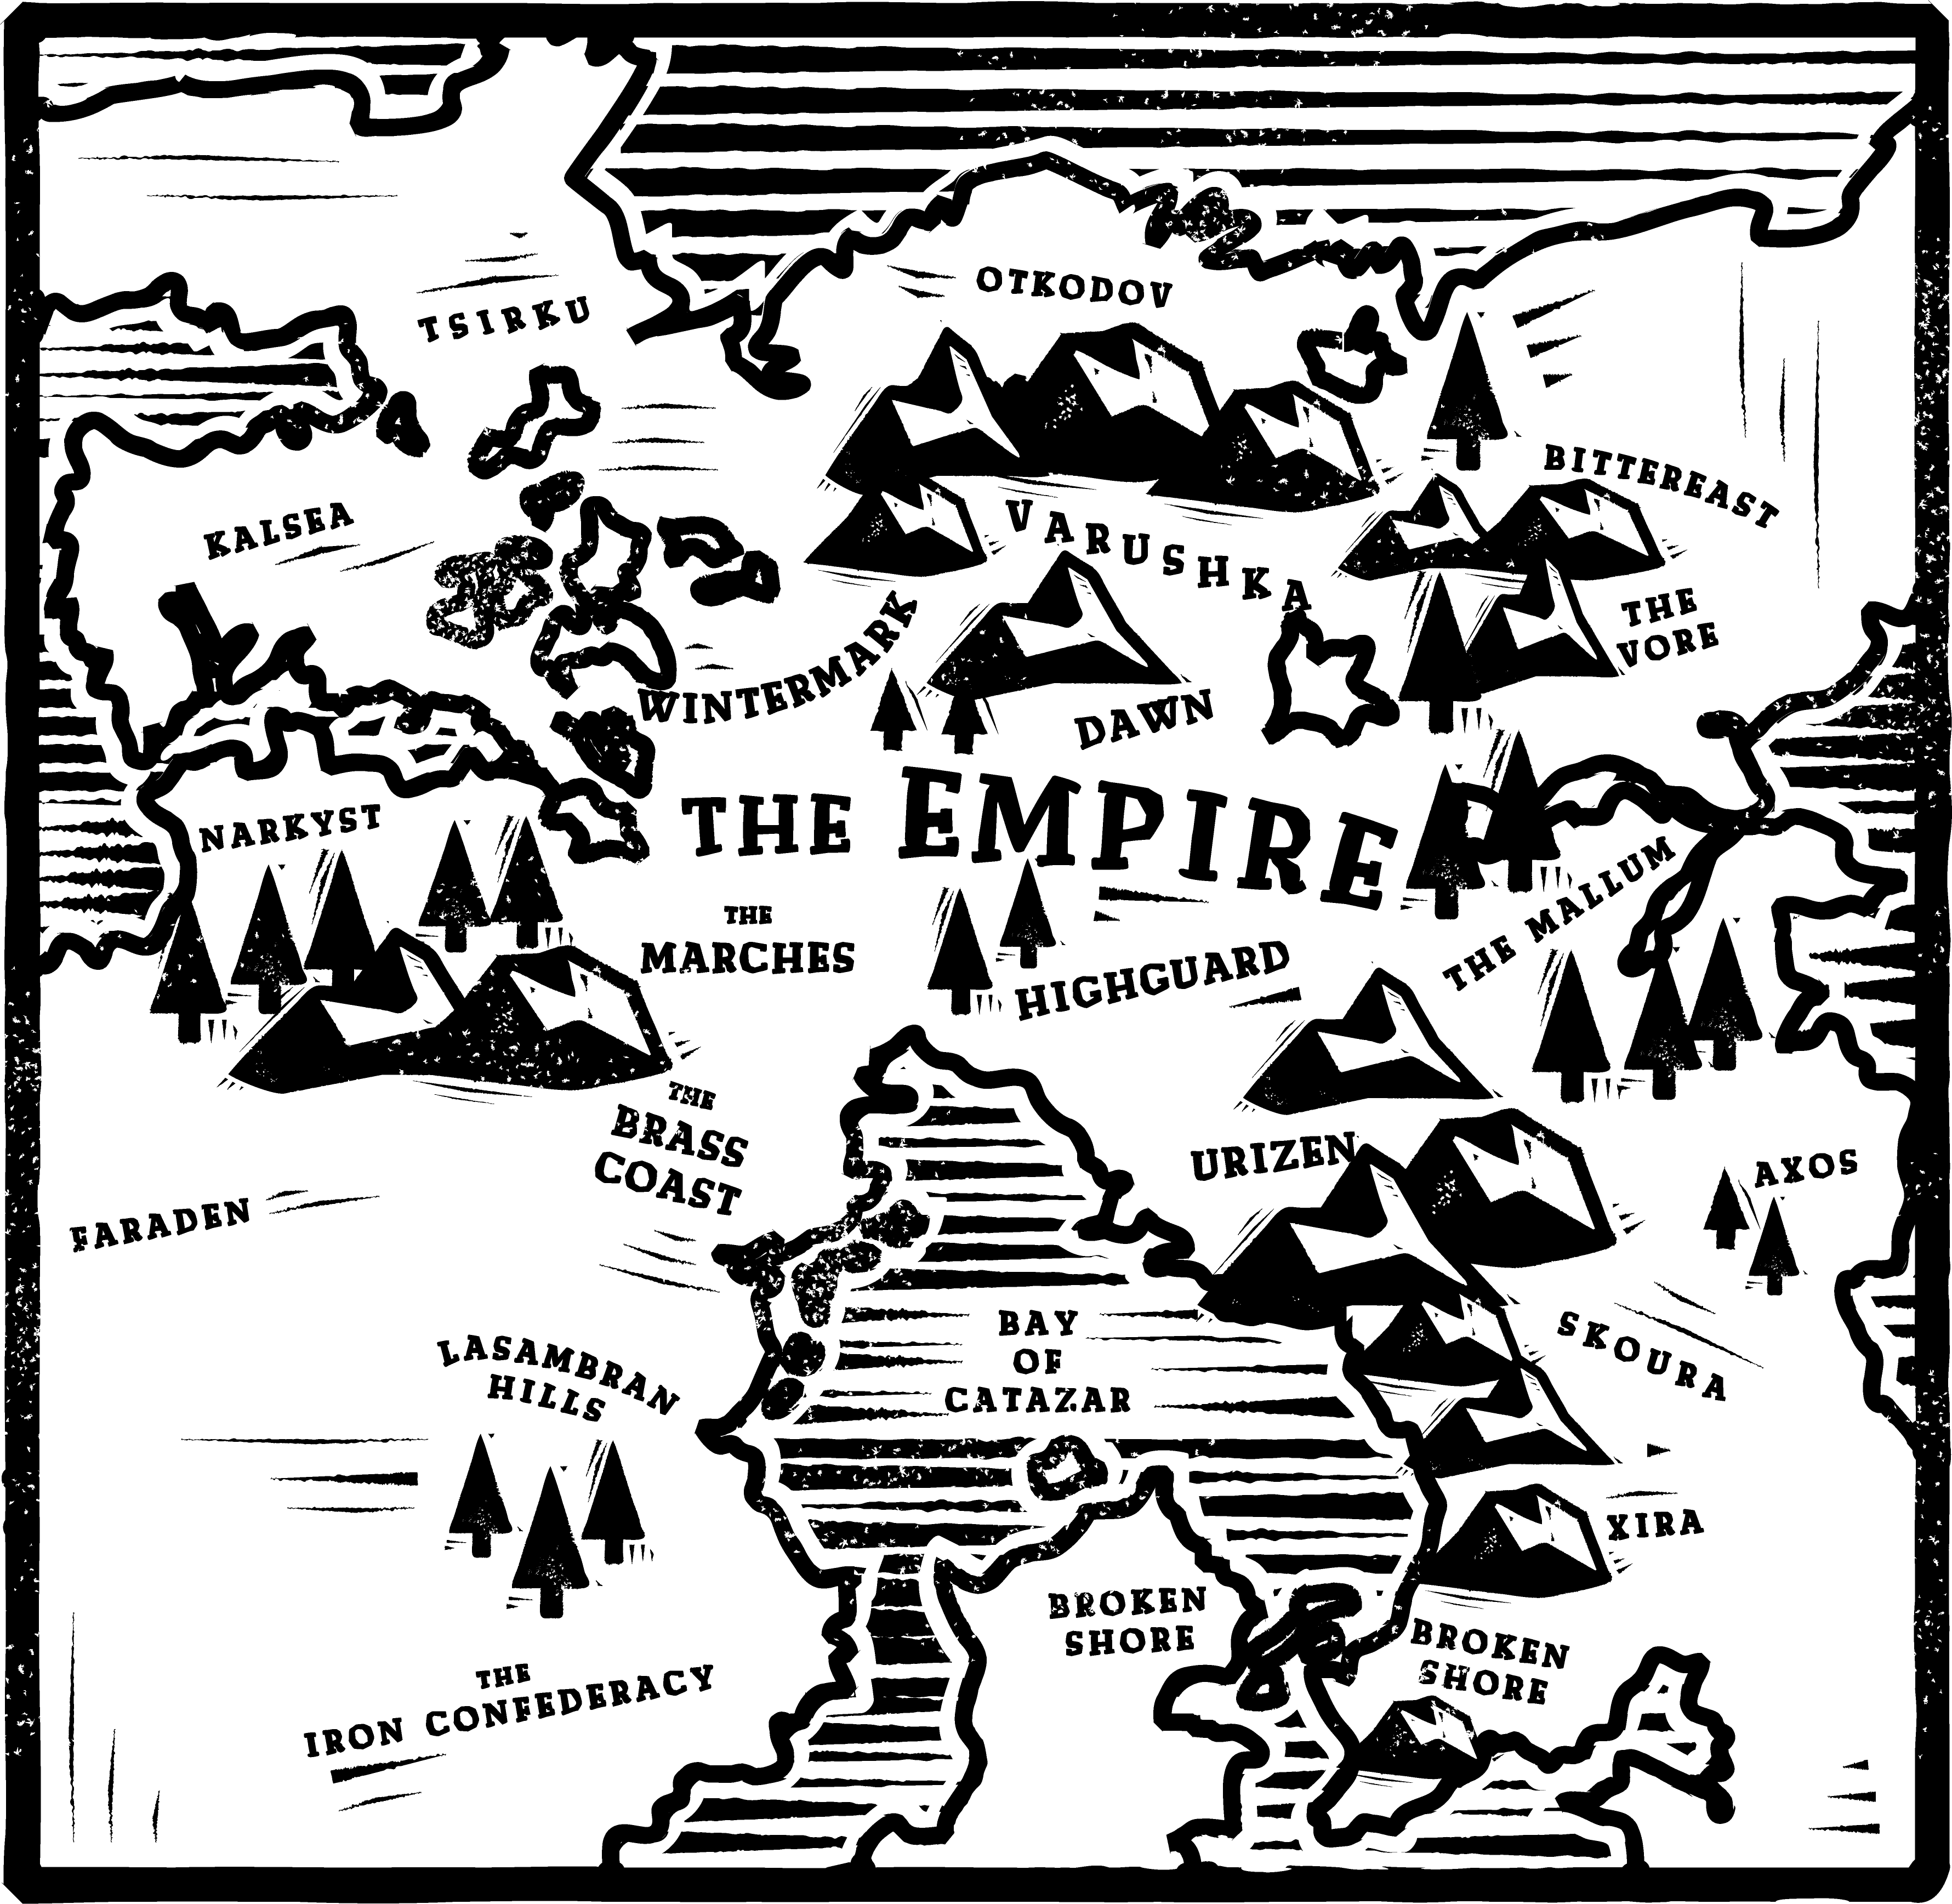
\includegraphics[width=0.9\textwidth]{encyclopedia/worldmap}\caption{t'empire and its neighbours}\end{figure*}
\paragraph{Forte Fidelis} old asavean for []. a fortification around \see{Hay} in \see{Mitwold}.
\paragraph{Freeborn} an inhabitant of t'\see{brass coast}.
\paragraph{Freemoor} a region in t'northern \see{Mournwold}, held by t'\see{Jotun}.
\paragraph{friar} a travelling monk
\paragraph{Golden Downs} t'region around \see{Hay} in \see{Mitwold}, containing the garrison \see{Forte Fidelis}.
\paragraph{good walder} paragon of prosperity. Probably an early landskeeper.
\paragraph{Grand Market} a market in \see{Meade} which takes place on the third weekend of each month and attracts traders from across the Marches and even occasionally from Wintermark to the north. 
\paragraph{granite} \see{white granite}
\paragraph{Graven} market town in \see{Bregasland}. Graven grew rich from Graven Rock, its high fields and mineral wealth. In happier times t'\see{Navarr} came here often, with news and trade-goods from far afield. Many's t'inhabitant here who started life far, far away, brought here by a Navarr Guide. Nowadays, it’s t'base of supply for t'castles and forts that defend Bregasland against t'\see{Jotun} in t'\see{Mournwold} and t'forests of \see{Liathaven}.
\paragraph{Gravenmarch} the region around \see{Graven} in \see{Bregasland}.
\paragraph{Greensward} the region around \see{Overton} in t'\see{Mournwold}, the only region in t'Mourn held by t'empire. Can also refer to t'Overton Monastery.
\paragraph{green iron} a gray metal, generally symbolised by a sword. Used by magicksmiths to create dyes or lightwight \see{magickal item}s that offer protection.
\paragraph{Green March} a region in t'\see{Mournwold}, held by t'\see{Jotun}.
\paragraph{Greywater} village in \see{Bregasland}, t'furthest west any wise Marcher will go. T'locals make their living primarily from eel-fishing, but since this isn’t a trade that leads to many exports, some of t'more daring amongst them will scour t'surrounding marsh for unusual plants and flowers. These are dried, and sold through t'markets at Meade. T'local grey water is not t'best water to drink, so there's a thriving market in pure water.
\paragraph{Grey Fens} The region around Greywater in Bregasland.
\paragraph{hallow} a ceremony that gives a magickal item an aura of \see{virtue}, affecting everyone bound to t'item.
\paragraph{Hay} a small rural town set amongst rolling field in southern \see{Mitwold}, near the border to the \see{Jotun}-occupied \see{Mournwold}. “The golden fields of Hay” appear in many a Marcher song.
\paragraph{Heath} a region in \see{Upwold}, containing the \see{Sutton Quarries} and bordering the \see{Mournwold}.
\paragraph{hearth magick} is a low-key everyday type of magick that keeps us being safe and prosperous. It is also important for keeping t'\see{Jack-in-chains} bound. Important elements of Marcher hearth magick are t'appropriate burial of Marchers in Marcher soil after \see{death} (cf. \see{Holberg}), and many elements of tradition, such as \see{poppet}s and seasonal festivals, grant t'Marchers persistent prosperity through hearth magick.\proverb{T'answer lies in t'soil.}
\paragraph{hedges} a line of shrubs and important marker of t'boundaries (\see{beater}) of fields and communities. As of new, it has become a tradition to bury dead \see{briar}s in t'brambles of hedges. \proverb{A hedge between keeps a friendship green.}
\paragraph{herald}
\paragraph{herb} in addition to herbs useful in cookery and brewing, imperial herb gardens grow five herbs with important applications in \see{medicine}. \begin{table*} \begin{tabular}{p{0.6\textwidth}} blue mazzarine to save a limb\\ grey bladeroot stems a weakness dim\\ red roseweald venom’s power breaks\\ true vervain body's healing wakes\\ though marrowort takes soldiers' pain\\ at battle's end they'll fall again\\ \end{tabular}\caption{medical herbs}\end{table*}
\paragraph{herding cats}
\paragraph{heresy} t'religious \see{crime} of willfully rejecting, or perverting, t'orthodox doctrines of t'faith as laid down by t'imperial synod, or actively teaching and promoting false doctrines.
\paragraph{highguard} t'\see{nation} that created t'imperial \see{faith}.
\paragraph{Holberg} t'easternmost city of t'League, notable for containing small enclave of Marcher soil in \see{league}, where Marchers were put to rest. T'establishment was necessary because t'bodies had been animated through a \see{winter} \see{ritual} to fight in t'liberation of t'city from t'\see{druj}, which interfered with Marcher \see{hearth magick} concerning \see{death} and awoke \see{Jack-in-chains}.
\paragraph{hunger} is a sign of lack of \see{prosperity}. Unfortunate Marchers are welcome to help themselves to t'fruits of t'grave-orchards, and many places such as monasteries give support to increase t'prosperity of downtrodden Marcher folk. In anvil, hunger can be alleviated by dining at tyke’s.\proverb{He who lives on hope, dies of hunger.}
\paragraph{husk} an animated corpse, eg. created by \see{winter} magick or \see{vallorn}. May need \see{burial} (cf. \see{Holberg}).
\paragraph{idolatry}t'religious \see{crime} of subsuming human will and destiny to any inhuman entity or force. This includes t'worship, veneration or exaltation of any such being or power.
\paragraph{ilium} star metal, a valuable material with strong magickal properties. Ilium can make magick effects permanent.
\paragraph{injury} there are several different conditions afflicting t'body to differentiate: a general loss in vitality; mortal wounds; terminal conditions; loss of limbs and some more special types of injuries. Other conditions, such as venoms or weakness, are discussed in t'essay on \see{medicine}. Ways of restoring injuries are different for different injuries. A general loss in vitality can be restored through an apothecary using a dram of true vervain, …. When a yeoman has lost all their vitality and suffered a mortal wound, causing them to bleed out, they can be helped by …. An individual who has lost all their vitality and has lost too much blood to ever recover should have no hope return to this life, but …. Destroyed limbs can be restored through …. Other, more serious injuries and traumatic wounds need t'attention of a skilled physick to be restored in a lengthy process, but a dram of marrowort can temporarily relieve t'pain.
\paragraph{insight} a priestly ceremony that allows a monk to discern a mark on someone's soul.
\paragraph{iridescent gloaming} t'wax from iridescent butterfly cocoons, generally symbolised by a butterfly. Used as colouring agent by magicksmiths who create \see{magickal item}s to enhance magick.
\paragraph{ISoM} t'imperial school of \see{medicine}, founded upon Marcher initiative, runs t'anvil field hospital. Anyone with an eager interest in t'medical arts of a chirurgeon, physick or apothecary will find much more intensive discussion of those matters in their wise library than in this loyal compendium.
\paragraph{Jack-in-chains} t'dark mirror of t'Marcher egregore \see{Jack-in-the-green}. Same name as an evil giant from a children's story, also kent as Jack-of-Irons or Bloody Jack.
\paragraph{Jack-in-the-green} t'Marcher egregore. As every \see{nation} of t'empire, all Marchers are bound to an egregore. Jack is a \see{beater} and has been around for generations. T'power of Marcher \see{hearth magick} keeps his dark counterpart, t'Jack-in-chains, bound deep in his core. If Jack-in-chains gets loose, he needs to be bound again by Marchers following their traditions, and innocent \see{soul}s binding him in place, just like in t'old legends we ken of t'Jack-in-chains. T'figures of Jack-in-the-green and Jack-in-chains may actually be older than t'formation of t'empire, for they have been part of legends even when t'empire was founded.
\paragraph{joshua benson} exemplar of vigilance, recognized by t'synod in 378. Known as “t'major”.
\paragraph{jotun} t'jotun are t'tribe of barbarian orcs that have captured t'\see{Mournwold} in 347. They are a warlike tribe that values strength-in-arms and fighting-spirit as their highest virtues; they love one-on-one fights, challenged by t'orc pointing at an opponent with their weapon and then raising their head up to show their necks to their opponent. Making a slashing or ripping gesture with their hand as they bring their head down with a snarl. This signal shows that they consider t'person they are looking at as worthy of honourable combat. T'target may return t'challenge, and engage t'jotun in single combat that ends until one warrior cannot continue. Jotun will usually accept a surrender unless they have reason to believe they are being tricked in some manner, and often allow injured opponents to retreat. They have also been kent to allow opponents who have fought bravely to gather their dead or injured. Warriors of t'jotun see little honour in killing t'weak or t'unarmed, and prefer to take them as thralls. Thralls are treated reasonably well by t'jotun; as long as they show proper respect to their overlords, they are usually left to their own devices. Many modern jotun thralls are t'descendants of humans taken in battle, and consider t'empire their enemy. T'jotun value courage, strength and martial prowess above other attributes. Their love of battle and emphasis on personal glory and honour, as well as their war-like traditions, means that many jotun warriors are a match one-on-one for their imperial counterparts. They do not throw their lives away, nor use their subject tribes as disposable troops, but they are invariably looking for a way to increase their honour, with an eye towards becoming ancestors when they die. T'only true dishonour most jotun recognise is showing fear in t'face of t'enemy, or striking a worthy opponent down by treacherous means. Jotun favour axes and hammers, both two-handed and coupled with a round shield. They tend to shy away from bows, and seem to have no appreciation for t'crossbow as a weapon of war – when it comes to ranged combat they prefer thrown axes or javelins. T'colour red appears to have totemic significance for t'jotun, and figures on most of their banners. \proverb{Better an honest enemy than a false friend.}
\paragraph{judgement} a decision of t'\see{synod}
\paragraph{Kallavesi} one of t'three traditions of \see{Wintermark}
\paragraph{King's Stoke} market town in \see{Upwold}, with a tower that existed before t'\see{March}, possibly built by t'Sentinel.
\paragraph{labyrinth}t'twisting realm of pure spirit that is integral to t'cycle of reincarnation, a core doctrine of t'\see{faith}. T'name is something of a metaphor for no mortal has been there to witness it, but t'journey from death to rebirth is neither simple nor instantaneous. Some spirits are said to wander between lives generations before being reborn, and some are lost forever. T'way of \see{virtue} teaches that living a virtuous life holds t'key to successfully traversing t'labyrinth of ages swiftly, safely and with t'purity of spirit that strengthens ties to past lives.
\paragraph{landskeeper's oath} T'oaths that landskeepers swear are often carved into a a tree, to bind them to t'land. By extension, a magick staff crafted from such a tree, which can allow a battle magickian landskeeper to bind enemies in place, is called a landskeeper's oath. \proverb{As easy to escape as a landskeeper’s oath.}
\paragraph{law} Marcher business is Marcher business, and should be conducted as such. Tradition has means to settle \see{boundary dispute}s, \see{sorcerer}s, and so on. But when individuals from elsewhere are involved in an affair, t'imperial code of law applies. This is often t'case for events related to a summit in anvil. Under imperial law, \see{foreigner}s have t'same protection as \see{citizen}s, though not t'same rights. \see{barbarian}s do not have those rights, quite t'opposite. Imperial law regulates crimes against people, crimes of position, crimes against t'state, civil claims and religious crimes. T'decision on guilt and punishment is made by a magistrate in a \see{trial}. T'corresponding tables list all criminal acts; It is possible for willing participants to give consent so that what would otherwise be crimes being committed against them are not. Attempting, ading or abetting of a crime is equivalent to committing t'crime under t'law. \begin{table*}\begin{tabular}{p{0.15\textwidth}p{0.85\textwidth}} Murder& action against a person with intent to kill them.\\ Manslaughter& against a person which results in someone’s death.\\ Assault& striking a citizen. (Lack of lasting injuries can make fights legal.)\\ Mayhem& maiming or mutilating a citizen.\\ Poisoning& applying a poisonous substance or effect to a citizen which causes them harm.\\ Imprisonment& Unlawfully detaining a citizen against their will. Suspects must be directly supervised during any period of lawful custody.\\ Malsanguino& Willfully preventing someone from receiving medical attention with t'intention of causing them harm.\\ Slavery& holding t'power of life and liberty over any person, including \see{barbarian}s. \end{tabular}\caption{crimes against t'person}\end{table*}\begin{table*}\begin{tabular}{p{0.25\textwidth}p{0.75\textwidth}}Theft& Dishonestly appropriating property belonging to another with t'intention of permanently depriving t'other of it.\\ Counterfeiting& falsifying, creating or amending of an imperial document or legal tender.\\ Criminal Damage& destroying or damaging any property either belonging to another citizen or to t'Empire. \\ Breach of interdict & Owning forbidden items and substances. This includes drake's eggs, vallorn seeds, t'Maggot's Talon wand, and t'poisons gutwrench, moon's poison, hunger of t'wolf, black gate and crimson gate. (for items interdicted by t'conclave, t'crime is against t'processes of t'state.)\\ Vallorn cultivation& Planting or tending vallorn is very likely to be interpreted to be vallorn cultivation, harvesting magickal ingredients from a naturally occurring vallorn pod may or may not be.\\ Trade of True Liao to foreigners& It is illegal to trade True Liao to anyone who is not a citizen.\\\multicolumn{2}{l}{\textit{Cases of negligence \&c. can be brought before forward in civil trials.}} \end{tabular}\caption{crimes against t'property}\end{table*}\begin{table*}\begin{tabular}{p{0.25\textwidth}p{0.75\textwidth}}Treason& Aiding barbarians, eternals, or foreign powers to act against t'interests of t'Empire. Committing an assault against t'emperor or empress. \textit{Only citizens and former citizens of t'Empire may be charged with treason.}\\ Impersonation of an Imperial Official& Falsely and dishonestly claiming to be a senator, civil servant, member of t'militia \&c., with intent to deceive.\\ Dereliction of Duty& Volunteering for an imperial duty and then failing to carry it out through neglect or cowardice. \textit{abuse of an imperial position is within t'remit of t'Synod.}\\ Vyig Membership & Membership in t'criminal organisation, or possession of Vyig tattoos. \end{tabular}\caption{crimes of position}\end{table*}\begin{table*}\begin{tabular}{p{0.3\textwidth}p{0.7\textwidth}}Contempt of Court& any behaviour which impedes t'proper operation of t'legal process, such as disrupting a trial, or failing to attend court.\\ Perverting t'Course of Justice& any behaviour calculated to unduly affect t'course of t'judicial process, such as bearing false witness, making false allegations, concealing offences or assisting others to evade arrest, interference with witnesses or evidence and evading, withholding or perverting a lawful punishment.\\ Subverting agencies of t'state& any behaviour which contravenes or subverts t'constitutionally protected procedures or powers of an agency of t'state. \\ Resisting Arrest& Any course of action with t'intent to oppose a lawful arrest.\\ Contravening a Declaration of Sorcery& as a declared sorcerer, owning crystal mana, performing rituals or interacting with Heralds and Eternals.\\ Improper placement of an aura on t'senate building& T'placing of an aura on t'senate building without prior explicit permission from t'Senate.\end{tabular}\caption{crimes against t'processes of t'state}\end{table*} \begin{table*}\begin{tabular}{p{0.2\textwidth}p{0.8\textwidth}}Idolatry& Subsuming human will and destiny to any inhuman entity or force. This includes t'worship, veneration or exaltation of any such being or power.\\ Blasphemy&T'denigration of t'Paragons and t'Paths of Virtue. This includes promoting False Virtues and t'teachings, or example, of False Exemplars or False Paragons.\\ Heresy& T'willful rejection, or perversion of, t'Orthodox Doctrines of t'Faith as laid down by t'Imperial Synod, or actively teaching and promoting False Doctrines.\\ Abuse of Powers& T'misuse, or abuse, of t'powers of a priest. This includes t'powers of t'Synod, as well as liao ceremonies.\\ Desecration& T'removal of spontaneously created auras such as legacies of ascendance to paragonhood. This includes such auras arising on areas, objects and people. \\ \multicolumn{2}{l}{\textit{Religious Crimes are tried by a magistrate but are raised by t'Imperial Synod.}}\end{tabular}\caption{religious crimes}\end{table*}
\paragraph{League} a \see{nation} of city-dwellers, trying to turn \see{Meade} into a city of their type. \see{Holberg} is t'easternmost city of t'league.
\paragraph{liao} a refinement of vinum, used in priestly ceremonies. T'very rare, pure liao allows citizens to experience visions of past lives.
\paragraph{lineaged} lineage means that a person is touched by one of t'\see{magick}al realms and can occur in many ways. T'table gives an overview of t'types of lineage and their associated realms. Parents with lineage often give birth to children with their lineage, while t'offspring of a human and a \see{herald} is always lineaged. It is also happens that fully human parents give birth to a lineaged child. Lineage can also occur for other reasons, for instance a child born in a primal forest under t'influence of t'realm of spring might become a \see{briar} in later life while a child born during a great famine when winter holds sway might be born a draughir. At certain times, t'flow of magick due to constellation on t'sky can influence t'occurrence of lineaged, either naturally or by making transformative magick easier. Many Marcher households are kent to not include any lineaged, despite appearance to t'contrary – denying t'merrow lineage of a household member by stating that he would be a mere human who is just feeling a bit blue –, or insist, for example, that their good cambions are spirited and energetic, whereas a cambion stranger would be seen as particularly conniving.\begin{table*}\begin{tabular}{lll} name& realm& trappings\\ \hline \see{briar}& spring& bark; volatile, impulsive \& restless behaviour\\ changeling& summer& pointy ears, antlers; bold \& self-confident attitude\\ cambion& autumn& curved horns; opinionated \& driven dominance\\ draughir& winter& pale skin, hollow eyes; cold \& hungry desire\\ merrow& day& gills, blue mottled skin; calm \& focused distance\\ naga& night& scales; relaxed \& passionate indulgence\end{tabular}\caption{t'lineages}\end{table*}
\paragraph{loyalty} a \see{virtue} \proverb{A chain is only as strong as its weakest link.}
\paragraph{magick} mostly refers to what magickians do, but there is also \see{hearth magick}. Every magickian is able to perform three basic magickal effects. Magickians can create bonds between citizens and magickal items or groups (banners, covens or sects) of imperial citizens bound by a common oath. They can detect and to some extent identify magickal effects such as enchantments on items or individuals they consider, a ritual being cast in their presence, or magickal items. When considering a precise location at t'sentinel gate, they can discern if there is a conjunction to that place; and if so, when it will open; how many people may pass through it; and any special circumstances that related to that conjunction. Finally any magickian can investigate and operate portals such as those bound to regios or t'\see{sentinel gate}, including traveling through, allowing eternals to communicate through, or tracing where they recently opened to. While some magickians extend this number of spells by other useful incantations that mend equipment or problems of \see{medicine} or can be used offensively, many magickians focus on joining covens to cast \see{ritual}s, such as t'mummery plays used to improve productivity of Marcher farms. Rituals always correspond to one of t'realms of magick, which are named (but at most metaphorically related to t'seasons of) \see{winter}, \see{spring}, \see{summer}, \see{autumn}, \see{day} and \see{night}. An overview over rituals a landskeeper might come in contact with is given in an \see{appendix}. For a given problem, a vigilant landskeeper may be well served finding out which realm is likely to be relevant and find an expert on that realm for deeper wisdom. \proverb{If all you have is crystal mana, every problem looks like a farm.}
\paragraph{magickal item} craftsmen can use t'rare materials orichalchum (o), iridescent gloaming (ig), beggar’s lye (b) ambergelt (a), tempest jade (j) green iron (g), dragonbone (d), weltsilver (w) to create magickal items. Such items retain their special function for 4 seasons, after which they have to be re-charged, essentially creating t'magick again from scratch. It does mostly take a magicksmith a full month to create an item; for such items as are empowered by skillful application of t'artisan’s craftsmanship alone, and not through t'magickal properties of their materials, it takes an artisan 2 full months. Personal magickal items can be armour, weapons or talismans (including shields). A magickian needs to create a bond between t'bearer and t'item, and every citizen can only have one bond of each of t'three types. Magick jacks or mithril mail can still be worn under good steel. In addition, a group can have a magickal banner, covenstone or reliquary, and such item can aid every member of t'group. T'late pete keeper of king’s stoke has analysed and composed a selection of inexpensive, useful equipment for t'soldiers of a Marcher household, which is reproduced here for convenience. \begin{table*}\begin{tabular}{l}bolstering bill – a dying comrade may be saved once a day. 6 g, 7 w.\\ butcher’s bill – cleave a foe in twain or bowl them down once a day. 8 o, 2 ig\\ warden’s bardiche (bill) – another surge of heroic might. 10g 3 a\\ reaving mattock (great weapon) – shatter an armament once a day. 7j\\ oathkeeper’s bow – another surge of heroic might. 8 g 5 a\\ biting blade – this side-sword will cleave a foe mightily once a day. 7 o.\\ stoutheart gambeson (light jack) – an extra degree of fortitude, slowing t'wearer’s bleeding. 2 months of a magicksmith’s time.\\ winter’s breath (light jack) – cure three of your wounds once per day. 5w 5a.\\ soldier’s harness (light jack) – t'yeoman soldier may suffer another blow before she falls. 8a\\ mediator’s mail (medium weight) – cure three of your wounds with heroic might. 2 months of a magicksmith’s time.\\ mithril shirt (medium weight) – t'yeoman soldier may suffer another blow before she falls. 2o 4a.\\ warrior’s plate (heavy steel) – t'yeoman soldier may suffer another blow before she falls. 2 months of a magicksmith’s time.\\ phial of t'sun – counts for t'herb of a physick’s choosing, once per day. No use in potions. 3w 3 a 2 b.\\ chrysalis pendant – may use heroic might to set a broken limb. 8w 5a 3b. Expensive but valuable.\\ bannerman’s band: you may save a dying ally through heroic might. you may also do this for free once a day. 5g 4a 5d. Highly effective, more so than a bolstering bill. Lets you use your own reserves too.\\ pilgrim’s shield: t'shield-bearer may suffer another blow before he falls. 2 months of a magicksmith’s time. User must be dedicated or anointed to a virtue.\\ alderman’s edge: a talisman allowing t'wearer to use a bill, greatsword or spear with t'ease of a weapons master. 8j 5d\\ bondring: you may bond to an ally as you would to a banner. you may heroically staunch their bleeding or cure a few wounds, once a day. 7d\\ wayfarer's pyx: when this reliquiary is \see{hallow}ed by a friar, t'ceremony lasts as long as t'item does. 2 months of a magicksmith’s time.\\ banner of t'bold: all characters bonded to this banner are brave in t'presence of even supernatural auras of fear. 2 months of a magicksmith’s time.\\ t'effects of various covenstones are far too specific to be listed here.\end{tabular}\caption{t'quartermaster's aide}\end{table*}\\
\paragraph{magnitude} is a measure for t'power of of a \see{magick}al ritual. Multiple landskeepers can cast a ritual together if they are in one \see{coven}, but a coven can only cast two rituals per day. [t'magick maths: mastery, lore, regio]
\paragraph{Maidenstone} an ancient dolmen in \see{Mitwold}. T'stone stands in a scorched area of land in a grove of ash trees. Every year before t'Spring festival t'farmers of t'area weave t'largest straw dolly known in t'territories. T'Straw Maiden, as t'creation is known, is 12 feet tall adorned with wild flowers with intricate patterns of vines woven into her skirt. T'Maiden’s skirt is hollow at t'base and she is placed atop t'dolmen. T'Landkeepers of t'area then bless t'Maiden in many nights of ritual. T'Maiden then stands in t'grove, visited by pilgrims who proffer food, trinkets and other offerings at her foot in t'hope that she may bring them some small favour. This continues until t'summer has ended. Mysteriously although t'Maiden has been exposed to all weathers and temperaments, she does not rot, blow away or decay in any way, staying as fresh and brightly golden as t'day she was placed upon t'stone. Then, at t'festival of Harvest there is another ceremony, t'culmination of which sees t'Maiden set alight, burning until there is nothing left. 
\paragraph{Maiden Downs} region in eastern \see{Mitwold}
\paragraph{major} (or mayor) 1. An old upwold word for steward 2. \see{joshua benson}, examplar of \see{vigilance}
\paragraph{mandowla} a legendary beast with a sturdy bear-like body with savage talons rather than claws and a head that resembles that of a giant owl with wide eyes and a savage beak. Often found in small family groups, they are omnivores – although with a marked preference for raw meat. They have a predator's cunning and are quite capable of attacking humans if they are disturbed or angered. They are most active at twilight, but have both excellent night vision and keen daylight sight. Common around upwold. These creatures are more dangerous than bears simply because they are so ready to attack and kill humans. They do not go out of their way to hunt humans, but if a family moves into an area containing a village, it will need to be dealt with. A small group especially one armed with long pole weapons should be able to bring one to bear and defeat it.
\paragraph{Marches} a nation, bound to t'egregore \see{jack-in-the-green}. \begin{figure*}\centering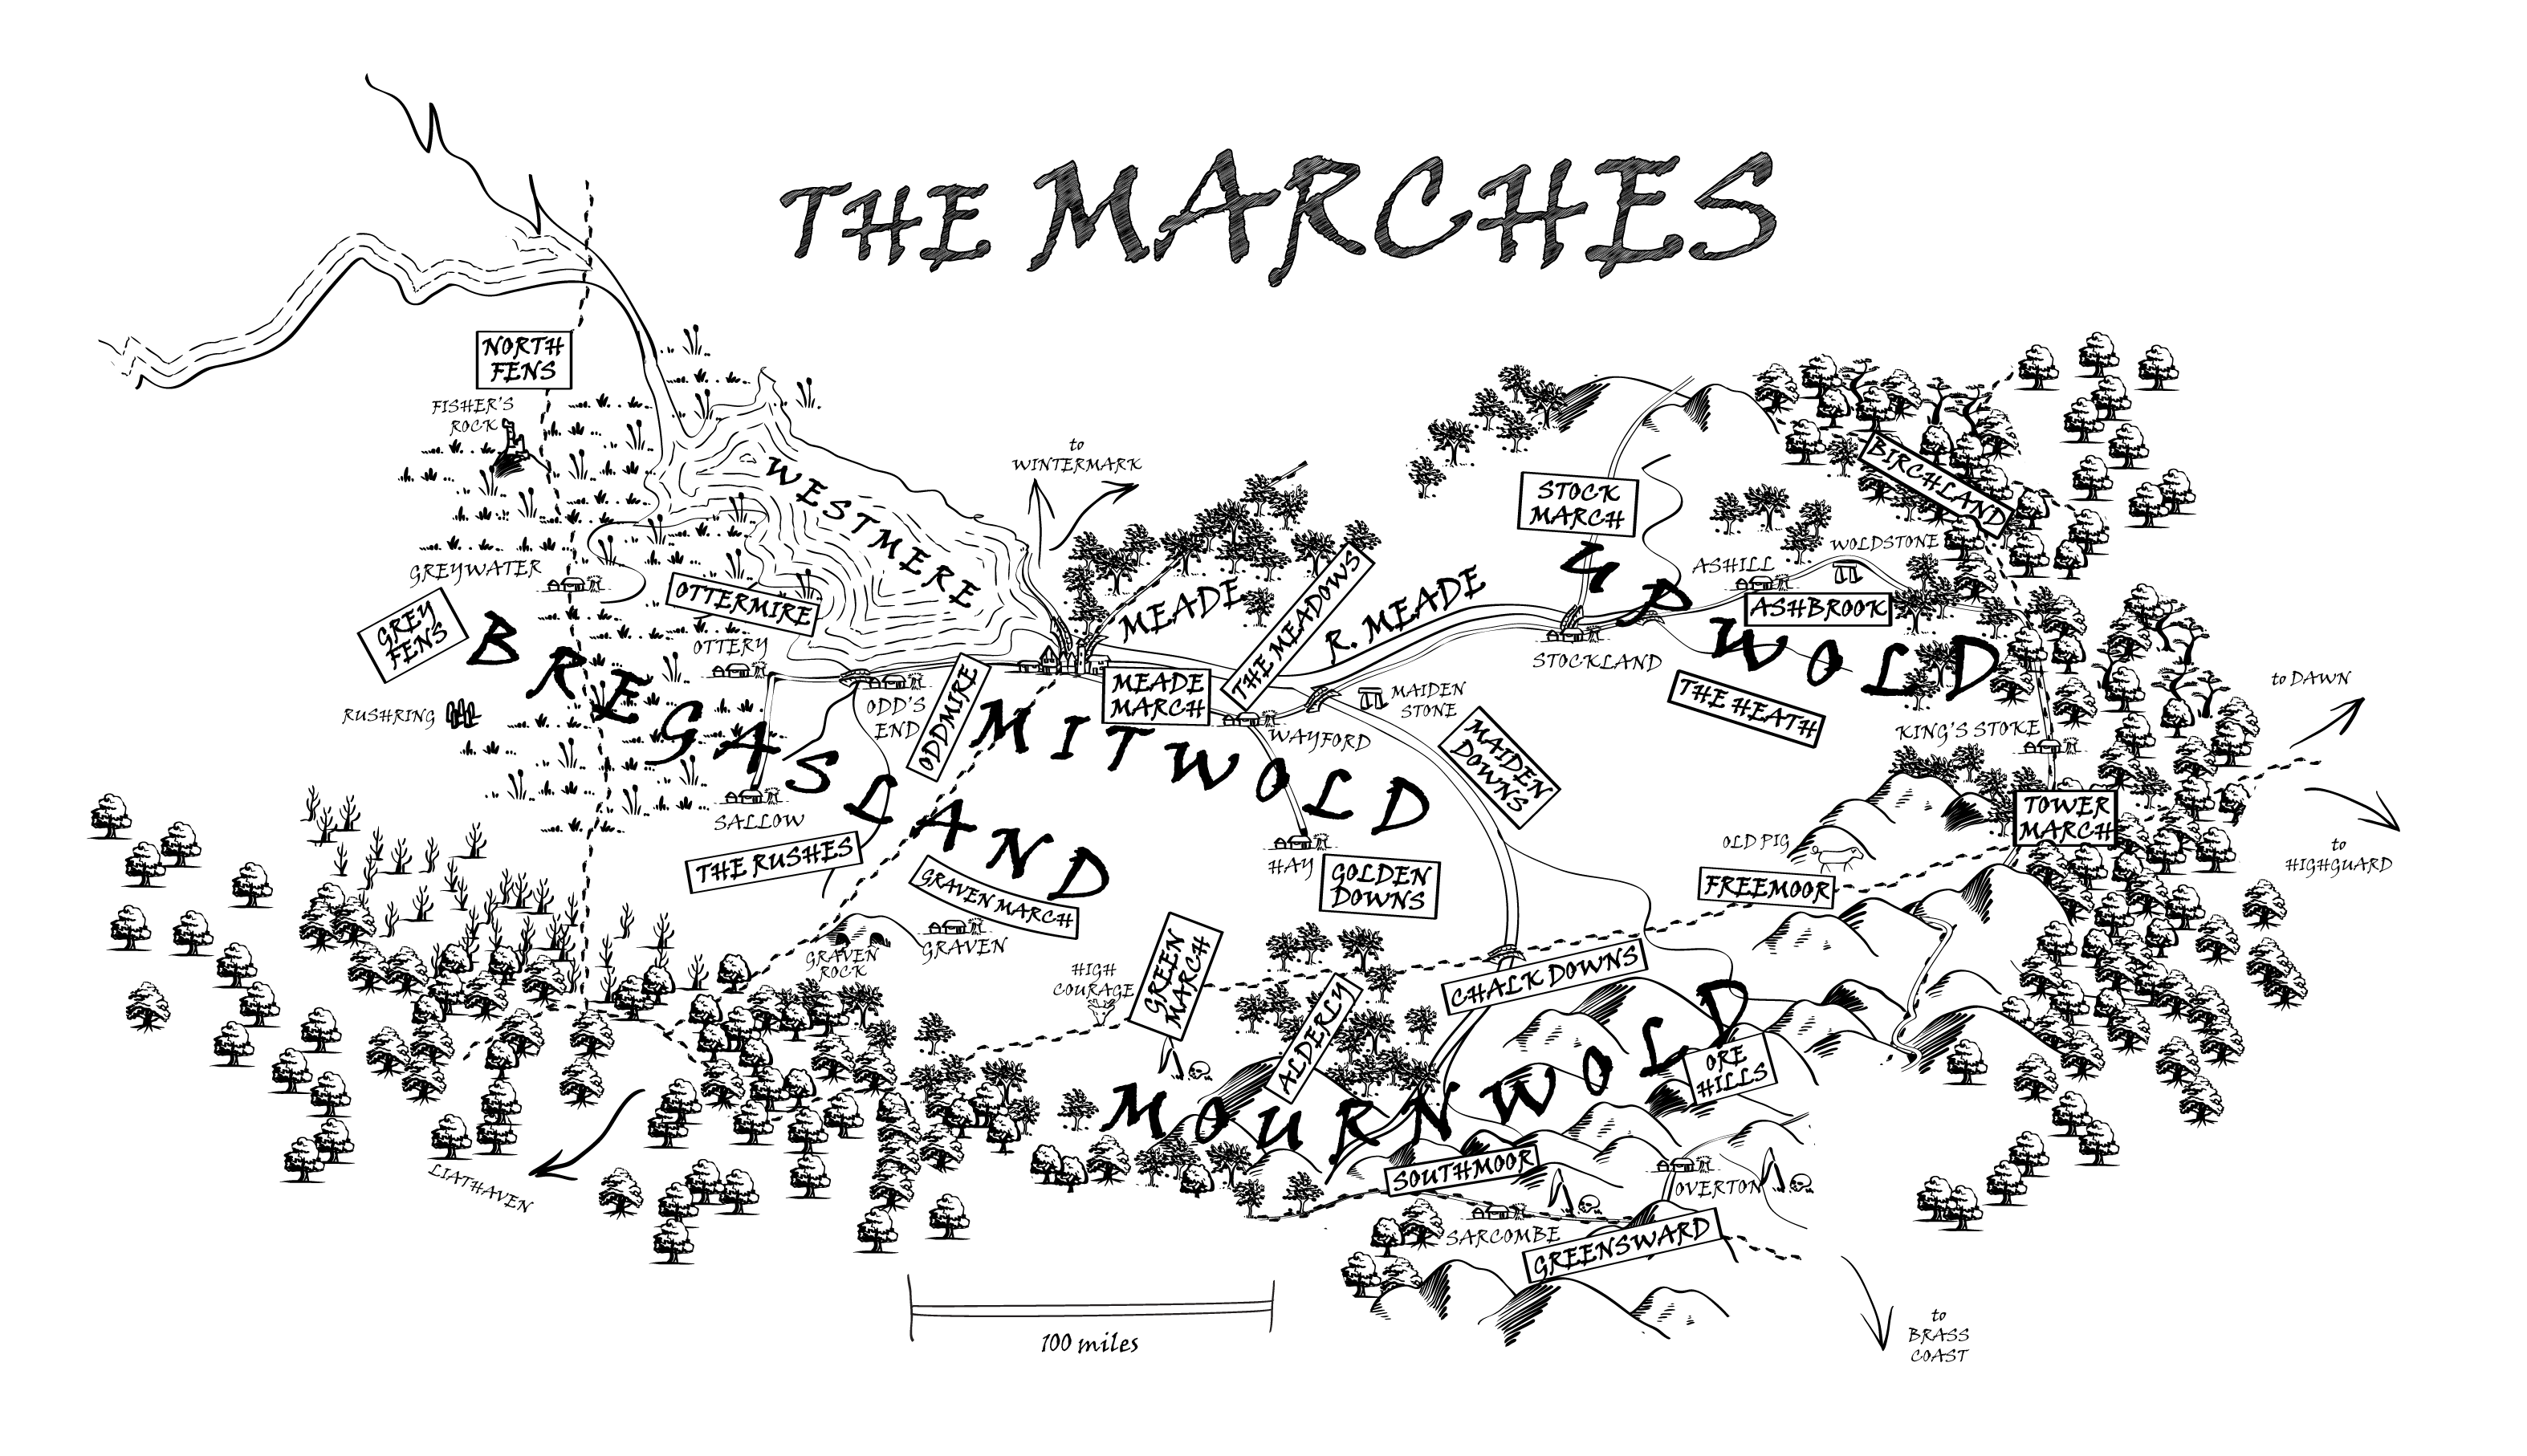
\includegraphics[width=1.1\textwidth]{encyclopedia/marches}\caption{t'Marches}\end{figure*}
\paragraph{March} t'rebellion of Marcher yeomen leaving Dawn; transferred: becoming a Marcher
\paragraph{marshwalker} a large semi-humanoid creature that appears to be made entirely of plant material, coated and held together with thick slime. Primarily found in marshy conditions, such as \see{Bregasland}, t'\see{druj} sometimes bring them along on battles. They are most dangerous when exposed to \see{vallorn}. One problem with marshwalkers is that, in their natural state, they are simply a colony of little slimy blobs that are virtually indistinguishable from t'mud in which they live. In this state they are no threat to anyone, being primarily concerned with eating small insects, fish and plants and splitting into more tiny, nonthreatening blobs. It is only when they feel threatened, when some biological urge inside them decides it is time to move, or when someone starts building a structure near or threatening their habitat that t'colony comes together to assume t'much more dangerous form of a wood-armoured humanoid. Their migrations often take them near human settlements. Attempts to divert a marshwalker exodus are complicated by their resilience, their resistance to fire (they are simply too damp to burn), and their ability to smash through most obstacles placed in front of them. A marshwalker is a major threat to a village, and several marshwalkers might threaten a small town. A well-equipped militia can probably drive a marshwalker off, but are likely to take serious injuries in t'process. A lone character can easily outpace one, and might be able to come up with a cunning way to divert one, but one-on-one will likely be quickly dispatched. 
\paragraph{materials} what a magicksmith uses to create \see{magickal item}s. \begin{table*}\begin{tabular}{lllp{0.5\textwidth}}name& shape&mark&effect\\\hline orichalcum&ingots of golden metal & shield& piercing; dissapating blows \\ tempest jade & chunks of green stone & lightning & decoration; polishing \\ green iron & ingots of gray metal & sword & lightweight protection; dyes \\ weltsilver & ingots of greenish metal & droplet & channeling energy; jewellery \\ ambergelt & chunks of red resin & wasp & healing, preservation; decoration \\ beggar's lye & bottles of tree ash & skull & caustic; changing material properties \\ dragonbone & sticks of marrow-clay & dragon & channelling bonds; clay-like shaping \\ iridescent gloaming & bottles of cocoon wax & butterfly & colour wash; enhancing magick \\ ilium & ingots of star metal & flame & making magick permanent \\ liao & bottles of liquid & labyrinth & priestly ceremonies \\ crystal mana & various crystals & certificate & casting rituals \\ \multicolumn{2}{l}{five imperial medical \see{herb}s} & certificate & \see{medicine}; \see{potion}s \end{tabular}\caption{trading commodities}\end{table*} \begin{figure}\centering
\includegraphics[width=2cm]{encyclopedia/greeniron} \quad 
\includegraphics[width=2cm]{encyclopedia/orichalcum}\caption{green iron (l), orichalcum (r)}\end{figure}
\paragraph{Meade} a big market town in Mitwold. Some misguided business owners from Meade would like it to become a \see{League} city. \proverb{A pig in t'house does not make a farmer}The largest settlement in t'Marches is t'market town of Meade in Mitwold. Crowded around t'mouth of t'eponymous river on t'shores of Westmere, Meade is not only t'spiritual and administrative heart for t'nation, it’s also a port whose ships deal in fishing, trade with foreign nations and sea defence against t'barbarians through Westmere and t'Gullet. It’s where Marchers from smaller towns often come to spend hard-earned coin, and more often than not plays host to exotic foreigners. T'Harvest’s End Festival sees Meade filled with folk from all across t'Empire, and it’s said that no-one sleeps there for a week. In t'wake of t'death of Empress Britta in 376YE, semi-organised groups of bandits began to prey on traders travelling by land from Meade. By order of t'Imperial Senate, in early 377YE a series of watchtowers and earthworks were constructed around Meade to help address this problem. T'works were overseen by Bridget Eastville née Talbot (senator for Mitwold) as part of a larger plan to provide protection to towns throughout t'Empire. While t'defences are not sufficient to qualify Meade as a true fortification, they have already helped reduce brigandry throughout t'territory. T'Bailiff of t'Grand Market has a small office in Meade, although most title holders spend little time there (apart from to oversee t'security of t'grand market on t'third weekend of each month). T'Bailiff is an Imperial title auctioned each Winter Solstice through t'Imperial Bourse that can be held by any citizen of t'Marches.
\paragraph{Meadmarch} t'region around \see{Meade} in \see{Mitwold}
\paragraph{Meadows} t'region around \see{Wayford} in \see{Mitwold}
\paragraph{medicine} there are several afflictions of t'body. In addition to \see{injury}, which is discussed in a separate section, age, venoms, weakness, and other effects can have an influence on a body. T'\see{ISoM}, running t'anvil field hospital, publishes more in-depths literature on medical matters. For t'vigilant landskeeper, t'conditions of venom and weakness and how to cure them will be most relevant. T'most likely effect of a venom is to dilute t'blood, speeding up bleeding and thus reducing t'time in which a citizen with a mortal wound can still be saved. Such venoms can be cured by a physician using 1 dram of t'\see{herb} imperial roseweald, by drinking a bloodhallow philtre \see{potion} (a red liquid with white particles), a magickian who has learned t'purify spell, or a \see{day} ritualist using t'\see{ritual} ascetic star of atun (m. 2); bearers of an abraxus stone or under t'effect of t'vitality of rushing water ritual are healed from venom whenever they are healed otherwise. Unnatural weakness can be removed by a physican using one dram of bladeroot, t'feverfail elixir (a flowery, grey sirup), a magickian who has learned t'purify spell, or a summer ritualist casting renewed strength of t'new day (m. 2). \proverb{Physick's faults grow orchards.}
\paragraph{militia} thee militia are vital to t'process of justice in anvil. They typically perform t'bulk of any investigation work and brief t'magistrates before cases go to \see{trial}. It is a constitutional obligation for a citizen who has been deputised into t'militia to carry out their responsibilities. In practice it would only be in exceptional circumstances that a magistrate would suborn a citizen into t'militia involuntarily. All serving members of t'militia have t'powers and obligations to take reasonable steps to prevent crime and maintain public order; to apprehend those suspected of crime(s) in progress and to bring them before a magistrate; and to report any crimes which require investigating to a magistrate. Magistrates will also appoint members of t'militia to investigate specific crimes (a case). Members of t'militia (and magistrates) may not enter a place of sanctuary without t'express permission of a priest who is responsible for it. Even if permitted to enter they may not arrest or otherwise interfere with anyone within who has been granted sanctuary. An accused may only claim sanctuary for a limited period, usually one hour. This period allows t'accused to make a confession and to ask a priest to attend them at trial so that a plea for clemency can be made on their behalf.
\paragraph{mithril} one of t'four strategical Imperial resources, distributed by t'bourse. Mithril is used to improve mines, mana sites and military units, and to create or supply armies.
\paragraph{Mitwold} t'middle Marcher territory, containing t'large town \see{Meade}. Mitwold's substantial \see{Westmere} coast, populated by small fishing villages along t'shore, gives way to fertile chalk-soiled downs further inland, with rich game-filled woodland and larger farms and market towns beyond. There's gold in t'soil of t'north-western portion of t'nation; t'gold of summer's harvest.
\paragraph{monastery} a household of monks.
\paragraph{motion} a decision of t'\see{senate}
\paragraph{Mournwold} t'southernmost Marcher territory, lost to t'\see{jotun} in 349. Originally t'name referred to t'sound of t'wind in trees and across t'craggy hills. Whearas Upwold and Mitwold in particular are known for their sprawling farms, t'rugged terrain of t'Mourn is perhaps better known for it's mines. T'hills are riddled with rich veins of green iron, and with mine workings dedicated to extracting that ore. Prior to t'invastion of t'Jotun, there had been a growing tide of dissatisfaction among professional miners that all political power had been vested in t'hands of those who owned farms. There were regular complaints that mine owners, like farmers and stewards, owned and worked t'land.
\paragraph{nation}one of t'10 composite people of t'empire: t'Marches, \see{Dawn}, t'\see{League}, \see{Varushka}, \see{Wintermark}, \see{brass coast}, \see{urizen}, \see{navarr}, \see{highguard} and t'imperial \see{orks}.
\paragraph{navarr} t'\see{nation} treading t'trods that reduce t'\see{vallorn}'s power.
\paragraph{night} 1: a time 2: t'\see{magick}al realm of passion, mystery and secrets
\paragraph{oak} 1: a type of tree 2: a \see{magick}al symbol and \see{constellation} of fortitude
\paragraph{Oddmire} t'region around \see{Odd's End} in \see{Mitwold}
\paragraph{Odd's End} A bustling fishing port with a chip on its shoulder against t'larger Meade, t'fisherfolk of Odd's End pride themselves on being first out to t'water, t'banner of Odd – a leaping salmon – raised above t'waves before their Meade brethren have untied from dock. Odd was a \see{pilgrim} of \see{pride}, and founded a monastery here, settling her folk on t'shore when t'Marchers first reached t'Westmere and declaring that this would be t'place where she would end her days. 
\paragraph{Ore Hills} A region in t'\see{Mournwold} held by t'\see{Jotun}, rich in \see{green iron}.
\paragraph{Ottery} small fishing port in \see{Bregasland} that trades t'produce of t'marshes to \see{Meade} and across t'Westmere to \see{Wintermark}.
\paragraph{Ottermire} T'marshy region around \see{Ottery} in \see{Bregasland}
\paragraph{orichalcum} a golden metal, generally symbolised by a shield. Used by magicksmiths to create \see{magickal item}s that pierce or dissapate blows.
\paragraph{orks} 1. A species 2. T'imperial orks, t'\see{nation} encompassing all ork \see{citizen}s of t'empire.
\paragraph{Overton} a garrison town, monastery and fortified manor in \see{Greensward} in t'\see{Mournwold}. Overton was a sheep-farming town and market set on a hill, until it became t'front line of t'war with t'\see{Jotun}. It has received strong support from League forces from Tassato. Since t'Senate negotiatied a ceasefire with t'Jotun, t'threat that t'armies of barbarians will sweep across Overton is held in abeyance. However, this has not prevented smaller bands of Jotun sweeping down into t'valleys of t'Greensward in search of easy riches. In turn, Imperial raiding forces often strike from Overton into t'Mourn.
\paragraph{Our Hills} \see{Ore Hills}
\paragraph{Pickham} a monastery dedicated to vigilance, located between \see{King's Stoke} and t'\see{Eastern Guard}. T'monastery was founded in memory of t'exemplar \see{Joshua Benson} and owns t'oldest Marcher-built tower in t'Marches.
\paragraph{pilgrim} a \see{dedicate}d layperson
\paragraph{poison} a dangerous and illegal \see{potion}, such as gutwrench, moon's poison, hunger of t'wolf, t'black gate or t'crimson gate.
\paragraph{poppet} every home in t'Marches has at least one straw dolly or poppet, made at t'time of harvest to bring good luck to t'house and ward off evil omens. These intricately twisted and knotted effigies of straw, corn, oats, rye, grass or rushes traditionally bind t'vitality of t'fields and bring their strength into t'home. Many Marchers carry their own small poppets for protection. In particular, every child is given a straw dolly of their own to help protect them from sickness, and an expectant mother will carry a poppet to ensure t'health of t'child. Touching someone else’s poppet can transfer good and bad between people, and should not be done. When t'season turns again to sowing t'seeds for t'new crop these poppets are laid on t'fields and ploughed back into t'earth, or cast into a bonfire, ensuring a bountiful harvest for t'following year. A landskeeper might employ a poppet in magick that binds or shares vitality or strength, such as granting potence of a band of yeomen. A \see{sorcerer} might use a poppet to steal t'strength of an enemy or an enemy's fields, binding it as they twist and knot t'doll until t'poppet is destroyed or a year has passed. A friar might bind some of t'\see{sin}s of a Marcher to a poppet, to be taken away by t'\see{wassail} fire, akin to a \see{wicker man}. To make a simple poppet, take a small bunch of stalks, around 8 inches in length, and strips of wool. Fold t'stalks in t'middle, and maybe bind them just below t'fold and tie them tightly. Around a half inch to an inch below your first knot, do t'same. Split t'bundle into four strands, which will make t'arms and body for your corn poppet. T'middle two will become t'body and t'outer two strands will become t'arms. Bend t'stalks that make your corn poppet’s arms and bind carefully with t'strip. Take a longer strip and tie it around t'neck of your poppet. Bind t'body pieces together and crisscross strips around t'body. Take strips and tie them around t'base of your corn poppet’s middle and body section. Split t'bottom of your poppet to form t'legs, just as you formed t'arms, and bind them. For making a poppet from corn husks, see t'figure.\begin{figure}\centering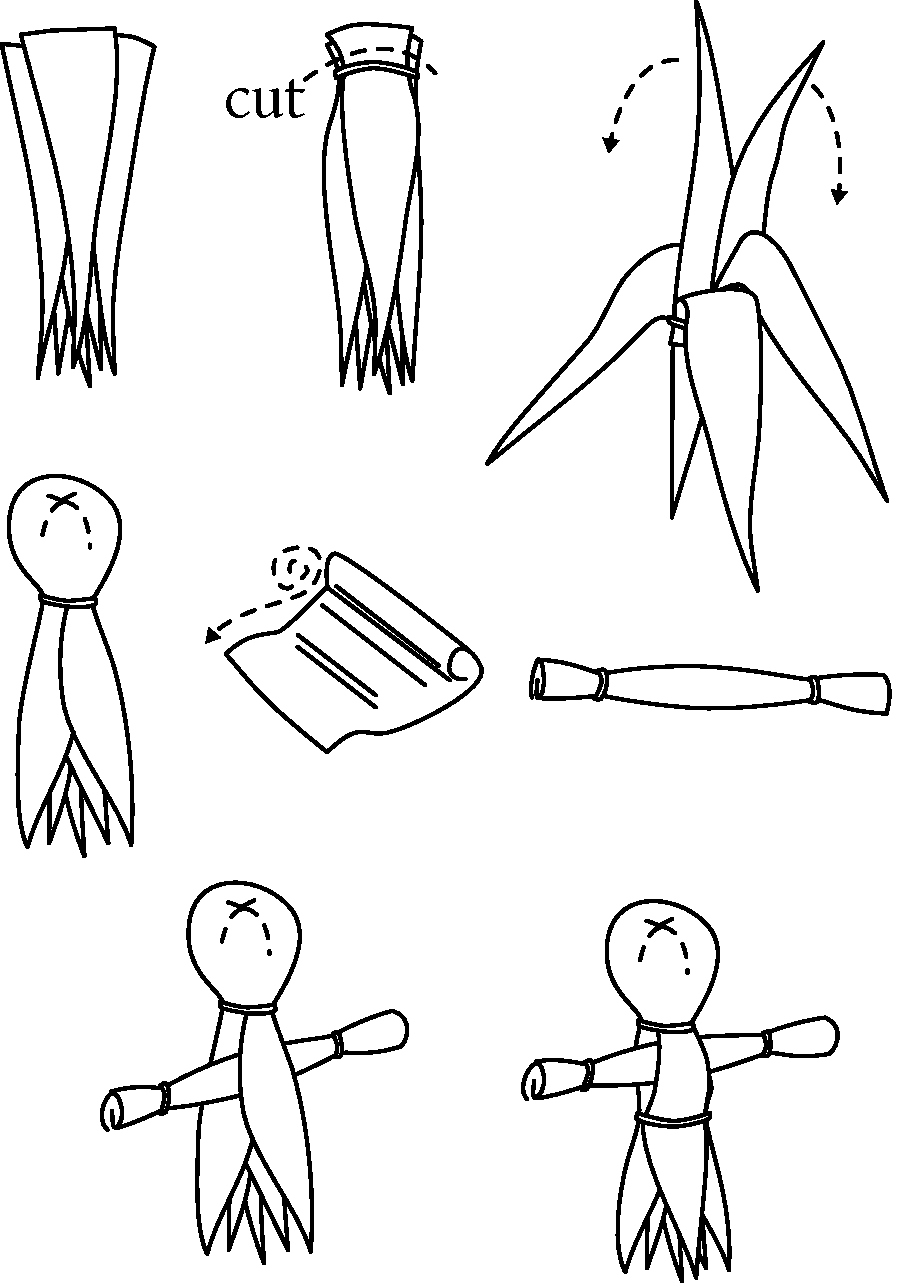
\includegraphics[width=5cm]{encyclopedia/poppet}\caption{making a poppet from corn husks*}\end{figure}
\paragraph{potion} brew of \see{herb}s with a supernatural effect. Every apothecary can create anodyne embrocation, bloodharrow philtre, elixir of life, feverfail elixir and ossean balm. For reference also listed are some other healing potions and poisons that need special attention. Some apothecaries can furthermore create potions that can influence citizens’ ability to perform rituals, religious ceremonies, heroic actions, \&c., but for those matters a vigilant landskeeper is better served finding a potions master or a tome on those items. \begin{table*}\begin{tabular}{p{0.15\textwidth}p{0.25\textwidth}p{0.35\textwidth}p{0.25\textwidth}} name &look &effect &ingredients \\\hline anodyne embrocation& numbing dark blue cream& temporarily numbs t'pain from traumatic wounds& marrowort, true vervain\\ bloodharrow philtre& spicy translucent red liquid& body is purged of venom, and of some minor poisons& imperial roseweald, marrowort& elixir of life& sticky blue-green translucent liquid& heals loss of vitality& vervain, cerulean mazzarine& feverfail elixir& flowery grey sirup& cools t'body and makes it regain strength& bladeroot, imperial roseweald& ossean balm& sandy blue salve& stabilises and heals a destroyed limb& cerulean mazzarine, bladeroot& gutwrench& viscous red-brown liquid& stomach feels on fire, possibly sweating, pain, weakness and venom& 2 imperial roseweald, 2 bladeroot, cerulean mazzarine& maledict's medicament& oily, deep crimson liquid & after some dizziness, quenches venoms out of t'body and strengthens t'body& cerulean mazzarine, bladeroot, imperial roseweald& tom drake's tea& viscous sweet-smelling yellow-green liquid& used to brew a pot of tea. Each person drinking a cup of t'tea is fully revitalised after fifteen minutes of rest.& marrowort, bladeroot& philtre of strength& blue sweet, spicy smelling liquid. & regain a level of heroic might.& vervain, bladeroot.& oakenhide tonic& golden boozy liquid, tastes of apples.& take an extra blow before you fall. Gain confidence.& vervain, bladeroot.& sovereign specific& pleasant, tasty, sparkly clear liquid& thoroughly heals t'drinker from all bad effects, including t'pain from traumatic wounds& imperial roseweald, cerulean mazzarine, vervain, bladeroot marrowort. & moon’s poison& indistinguishable from water& a growing chill and numbing throughout all t'body, reduced movement, coma, reanimation as a flesh-hungry zombie bent on killing and devouring t'living. T'wrong antidote speeds up t'process.& 3 marrowort, 3 cerulean mazzarine, 2 vervain, 2 bladeroot.& hunger of t'wolf& indistinguishable from water& a growing heat spreading through t'body, extremely short temper, voices urging them to kill everyone around. T'wrong antidote speeds up t'process.& 4 imperial roseweald, 4 vervain, 2 bladeroot.& feast for t'crows& lumpy red balm like rotting meat soaked in blood.& takes all vitality and delivers a fast death. T'only antidote for hunger of t'wolf and moonish slime.& 4 marrowort, 4 cerulean mazzarine, 3 bladeroot, 3 imperial roseweald, vervain. & t'black gate& indistinguishable from water& dizziness, weakness, increased confusion, random pain, growing awareness of own death, hallucination of loved ones or dead relatives. \see{weakness}, agonising seizure, death. T'wrong antidote speeds up t'process.& 4 bladeroot, 3 vervain, 3 marrowort.& t'crimson gate& indistinguishable from water& thirst, fever, agonising pain in joints and muscles, coughing blood, growing awareness of own death, venom. Blood from t'eyes and nose, death through own blood. T'wrong antidote speeds up t'process.& 4 imperial roseweald, 3 vervain, 3 cerulean mazzarine.& t'silver key& grey, resinous solution& uncontrollable cough, vomiting until stomach is empty. Loss of consciousness. Antidote to t'assassin’s gate poisons.& 4 imperial roseweald, 4 bladeroot, 4 marrowort, 2 vervain, 1 cerulean mazzarine.\end{tabular}\caption{relevant potions}\end{table*}
\paragraph{pride} a \see{virtue}\proverb{Pride in small things, loyalty to great ones.}
\paragraph{Pride of t'Marches} \see{Mitwold}
\paragraph{prosperity} one of t'seven \see{virtue}s. \proverb{Easy come, worth less.}
\paragraph{proverbs} provide \see{wisdom} and guidance for all honest Marchers. A collection of well-kent proverbs is included in t'appropriate places in this book. \proverb{War is a thrice-ploughed field.}
\proverb{One boy’s a boy, two boys is half a boy and three boys is no boy at all.}
\proverb{Liars and gossips sleep in t'same bed.}
\proverb{T'best patch is of t'same cloth.}
\proverb{T'apple never falls far from t'tree.}
\proverb{A bird in t'hand is better than two in t'bush.}
\proverb{T'chick needs space to spread its own wings.}
\proverb{What is bred into t'bone will never get out of t'flesh.}
\proverb{Shut t'stable door when t'ox is stown.}
\proverb{Safe as a thief in a mill.}
\paragraph{right of witness} synod priests are responsible for t'spiritual wellbeing of t'empire and are empowered to witness or observe all aspects of t'bodies of state in function. In practical terms, it guarantees t'right of synod priests to access t'senate public gallery, even if t'senate have called for a closed session and cleared citizens from t'public gallery; observe t'bourse private member's auction; be present in t'military council tent during meetings of generals. (except senators, who are forbidden from entering or being present during t'meetings of t'military council); be present at a meeting of t'conclave in t'hall of worlds. T'conclave has no responsibility for allowing non-magickian priests to reach t'hall of worlds, and have repeatedly pointed out that a magickian who is a priest has every right to attend a conclave meeting anyway. T'main use for t'right of witness in t'conclave is to observe t'election of t'grandmasters of t'orders. Traditionally, t'right of witness is also extended to t'relevant bodies in t'nations, such as t'meetings of stewards, captains and landskeepers in t'Marches. Refusing a member of t'synod t'right to witness is a crime against t'state under t'\see{law}. \proverb{Truth has no livery.}
\paragraph{ring} t'smallest coin, used to be t'value of a ring of \see{illium} in ages gone by. 20 rings make a \see{crown}, and 160 rings make a \see{throne}. \proverb{Take care of t'rings, and t'thrones will take care of themselves.}
\paragraph{ritual} a powerful procedure creating a \see{magick}al effect, such as an \see{enchantment} or \see{curse}. Some relevant rituals are listed in an \see{appendix}.
\paragraph{rough music} making a loud noise around someone \see{sin}ful, such as a \see{sorcerer}, until they give up their leave or change. \proverb{When a dog barks, you don't bark back.}
\paragraph{Rushes} t'marshy region around \see{Sallow} in \see{Bregasland}.
\paragraph{Rushring} A partially-submerged stone circle in t'Grey Fens in \see{Bregasland}. t'ring was t'notorious site of a number of ritual killings in 365. 
\paragraph{Sallow} a village in \see{Bregasland}. Sallowfolk keep themselves to themselves to a degree found off-putting even by other Bregaslanders. T'people of Sallow deal in cutting and drying rushes that are shipped to t'other towns of t'Marches for roofing. 
\paragraph{scarecrow} a humanoid doll made from straw, wood and clothes. Scarecrows have a protective function according to \see{hearth magick}, similar to \see{poppets}.
\paragraph{senate} t'primary legislative body for t'empire, elected by t'\see{citizen}s. In t'Marches, t'steward who can unite t'group of stewards and yeomen behind himself owning t'most land gets to select t'senator. Different stewards can oppose each other, even though they might nominate t'same individual as senator.
\paragraph{sentinel} a \see{paragon} of \see{vigilance} who built watch towers all over t'empire, such as t'eponymous one in Stoke. \proverb{If you want to hold t'land, first build a tower.}
\paragraph{sentinel gate} a \see{magick}al portal connected to t'imperial regio in anvil. Every magickian has t'skills to discern its conjunctions and operate it if a conjunction is happening.
\paragraph{shriven}\see{shriving}
\paragraph{shriving} t'process of basic shriving is simple. A monk who is willing to take on a Marcher’s faults or sins hears a confession. This can also be part of a preparation of a \see{clemency} plea in a trial, before t'execution of a criminal, before a dangerous battle, or on t'bedside of a Marcher on t'door to \see{death}. T'confessor should confess freely and without restraint, when he is told that t'monk is willing to shrive them. Whilst she listens, she weaves a poppet of straw, symbolically taking on part of his sin and embodying it in t'poppet. Once he has finished his confession and t'poppet is complete, she may offer a benediction of t'way such as this: “may t'way guide your footsteps on t'earth, ambition grant you t'will to strive, courage give you t'strength to act, loyalty cleave you unto your fellows, pride inspire you to accept your past, prosperity let you feast on t'fruits of your toil, vigilance keep you alert against falsehood, and wisdom keep you free of folly. May your sins be shared, your burdened halved, and your spirit guided by t'virtues.” she may also spend t'confessor an \see{anoint}ment. Once this is done, t'shriving is completed, and t'poppet should be burned at wassail along with offerings to atone unvirtuous deeds.
\paragraph{shunning} refusing to acknowledge t'presence of an individual, ostracising them. Wicker men and such like must also be shunned. \proverb{Make yourself useful, or make yourself scarce.}
\paragraph{sin} a transgression against virtues or traditions. \proverb{lost time is never found.}
\paragraph{sorcerer} someone using magick for \see{sin}ful purposes. T'\see{conclave} can declare someone a sorcerer, prohibiting them from magick under t'\see{law}. \proverb{dark minds find dark places to do dark deeds}
\paragraph{soul} \see{virtue}s \see{doctrine}
\paragraph{Southmoor} A region in t'\see{Mournwold} controlled by t'\see{Jotun}, containing t'ruins of Sarcombe.
\paragraph{sport and games} tug-of-war, foot-t'-ball \proverb{Don't mind t'rules, mind t'winning!}
\paragraph{spring} 1: a season 2: t'\see{magick}al realm of t'primeval force of life and growth.
\paragraph{Steinr} one of t'tree traditions of \see{Wintermark}
\paragraph{steward} a yeoman leading a household
\paragraph{Stockland} A sprawling town in western \see{Upwold} known for its sheep and cattle markets. Stockland ale is exported around t'Empire – not because it's particularly good, but it is recognisable, and can bring a lump to t'throat of t'homesick Marcher. 
\paragraph{Stock March} t'region around \see{Stockland} in \see{Upwold}.
\paragraph{Stoke} 1: a tower 2: \see{King's Stoke}
\paragraph{Suaq} one of t'three traditions of \see{Wintermark}
\paragraph{summer} 1: a season 2: t'\see{magick}al realm of might and majesty
\paragraph{synod} t'governing body for matters of \see{faith}, where all priests with a congregation have voting rights.
\paragraph{taint} a wild growth of dangerous supernatural and exotic plants where a \see{briar} was buried.
\paragraph{tempest jade} a green stone, generally symbolised by a bolt of lightning. Used for decoration and polishing by magicksmiths creating \see{magickal item}s. 
\paragraph{throne} 1: t'constitutional body of t'empress 2: t'largest denomination of money, equivalent to 8 \see{crown}s or 160 \see{ring}s. A well-run farm makes a few thrones a year, and wains of \see{mithril}, \see{white granit} and \see{weirwood} are traded with thrones.
\paragraph{thule} t'thule are inscrutable northern orcs, lead by \see{ritual}ists and fielding husks and fearsome beasts of war. Coming from t'resource-poor north, they are stripping dead enemies, invaded regions and captured territories of anything valuable. Some of these resources are being used to reinforce their armies, but t'lion's share is being sent north. Fighting against t'thule is fierce, especially since t'disastrous death of empress britta and most of her court. T'thule favour dark, hooded robes and cloaks, emphasizing their size and bulk with fur pelts over their shoulders. Thule consider a dark blue hue to be fortunate and revere dragons and wyrms as totemic beasts full of potence and cunning.
\paragraph{Tower March} t'region around \see{King's Stoke} in \see{Upwold}.
\paragraph{traumatic wound} any extraordinary type of \see{injury} that is not just a general loss of vitality due to blows with weapons including mortal wounds, or loss of function of limbs. A physick will be able to diagnose and right traumatic wounds.
\paragraph{trial} trials settle disputes of law. They are presided over by a magistrate. It is their role to run trials in a manner which is expeditious and just. Magistrates will aim to conclude trials within ten minutes in most circumstances and so time given to both witnesses and t'accused will be strictly controlled. T'accused will be presented before t'court. T'accused may be accompanied by a priest (if they intend to plead guilty and ask for clemency) or possibly by a friend or legal advisor. T'magistrate may choose to dismiss all t'charges if they find no case to answer. Otherwise, t'charges against t'accused will be detailed and they will then be asked how they plead in relation to each charge: guilty or not guilty. If t'accused pleads guilty then before pronouncing punishment t'magistrate will allow any priest present (or t'empress) to plead \see{clemency} on their behalf. Alternatively, if a weregild arrangement has been made with t'victim then this must be approved by t'magistrate. T'magistrate may also investigate and consider any other pertinent evidence or testimony prior to sentencing. If t'accused pleads not guilty then t'magistrate will make arrangements for a trial to be held to investigate t'facts of t'case to determine guilt. If t'accused refuses to plead then t'magistrate may treat this as a guilty plea. In either case a plea for clemency will not be permitted. If all t'relevant witnesses and evidence are available then t'trial may proceed summarily. Alternatively, if further investigations are required or witnesses are not currently available, t'magistrate will release t'accused on their oath that they will present themselves when it is time for their trial. Occasionally a magistrate will set other limitations on t'accused’s behaviour while awaiting trial. Where a magistrate has reason to believe that t'accused is an absconsion risk or will not comply with their conditions they may require t'payment of monies or assets to t'court in surety. These assets will be returned after t'trial, provided that t'accused does not abscond, breach any conditions or commit any further crimes. If an accused absconds then t'magistrate may try them in their absence. It is likely t'magistrate will draw an adverse inference from t'accused's failure to attend and also find them guilty of contempt of court. Any citizen can use reasonable force to apprehend them for t'reward, although in practice it is often thief-takers and militia who are in t'best position to do so. Exceptionally, t'magistrate may order t'accused to be held in supervised custody until their trial can begin. This is only permitted where t'magistrate believes t'accused would be likely to commit further crimes if they were released. If so, t'trial must be carried out as soon as reasonably practicable. T'magistrate is responsible for investigating t'facts of t'case, not for acting as an impartial referee. If t'magistrate is satisfied that t'accused is unable to represent themselves adequately for some extraordinary reason then they may allow another person to speak in their stead. This does not exempt t'accused from t'requirement to answer any questions put to them by t'magistrate. Judgement is made by t'presiding magistrate. Occasionally a magistrate may ask one or more of their peers to sit with them in judgement over a particularly difficult case. T'law allows magistrates to accept any evidence, including hearsay. T'minimum persons required to be present for a trial to be valid are t'presiding magistrate, and at least one other person. T'accused should also be present if possible, but may be tried in their absence if they abscond. Magistrates may choose to try all of those accused in connection with a particular crime or crimes at t'same time. This is particularly likely where a criminal conspiracy by a group of individuals is suspected. Where there are multiple offences which might apply to t'accused t'magistrate is only required to set out t'most serious charge(s). This does not prevent t'accused from being found guilty of a lesser related offence. If found guilty, t'punishment will also take into account any relevant lesser offences where appropriate. When determining t'accused's punishment t'magistrate will take into account t'seriousness of t'crime and any mitigating factors, for example presented by a priest in their plea for clemency.
\paragraph{trogoni} humanoid creatures with insect-like traits that live deep underground. They attack mana sites, consuming t'mana crystals and feeding on t'\see{magick}al flows. A single trogon is usually a match for an armoured warrior or two, with its tough carapace and savage rending claws.
\paragraph{upwold} t'easternmost Marcher territory, fortified.
\paragraph{urizen} a \see{nation} of kenning magickians.
\paragraph{vallorn} t'vallorn appeard when terunael, an empire from \see{navarr}i prehistory, fell. From t'hearts of their cities spread, a sick, infectious wave of life (\see{spring}) that crumbled stone, shot great trees up through streets and buildings, and warped what it found. Around t'core of each city areas of spring appeared, resistant to all efforts to destroy them. These were named vallorn. Inside them are monstrous plants, t'spores of which mutate living creatures that are exposed over many months. T'air within t'vallorn weakens those who enter, like venom. No complete catalogue exists – some things appear simply to be diseased, misshapen forest creatures, or mutated humans and orcs. Some seem to be plants, sporting a mass of tangled thorns or possessing abilities that make them dangerous to travellers. A common threat to those who venture into those areas where t'vallorn is strong are t'vallornspawn husks (animated corpses). That being said, there are non-vallorn spring monstrosities like marshwalkers or trogoni. It is important to remember that they behave basically like animals: show no fear, back off slowly and calmly, don't offer violence, don't block exits, don't bring yourself to their attention if you can help it, and \emph{do not play dead}. Climbing a tree may get you eaten by a tree.
\paragraph{Varushka} a \see{nation} in t'far north.
\paragraph{venom} many poisons (such as some \see{potion}s and t'mists of t'\see{druj} and \see{vallorn}) dilute t'blood, making someone on t'verge of death bleed out even faster. Ways of alleviating this are listed in t'essay on \see{medicine}.
\paragraph{vermin} locusts: if you catch some of t'locusts and burn them, t'others will be stupefied by t'smell: some will die, while others will fold their wings and wait to be caught, or will be killed by t'sun. This arises from antipathy. Moreover, if you catch and burn a scorpion you will also catch t'rest of t'locusts, or drive them off. Weasels: they say that if one catches one of t'weasels, cuts off its tail or testicles, and lets it go alive, one will not find any more of them afterwards on t'same farm. House mice: house mice are killed if you put down black hellebore with barley meal. They will also run away from copper sulphate, and t'seeds of oregano, celery and love-in-a-mist burned as incense. you can also employ such means as help against rats. Field mice: some farmers in Mitwold have succeeded by blocking t'holes with daffodils, so that as t'field mice hurry to get out they will take t'leaves with their teeth. When they bite them they will die. Foxes: a fox will not bite any bird under whose wing you have fastened wild rue. Snakes: no snakes will enter t'farm if you plant wormwood or mugwort or southernwood around t'farmstead; you will drive away those that are already there if you make smoke with white lily root or stag’s horn or goat’s hoof. Snakes will not trouble t'pigeon-house if in its four corners you write adam: if it has windows, write it at these too. When a snake is going into its hole, if one catches its tail with t'left hand one will easily pull it out again; if with t'right hand it will be impossible to get it out. Either it will escape, or t'tail will break off. Scorpions: if you rub your hands with radish juice, you can pick up scorpions and other such creatures without fear and without danger; and radishes, placed on scorpions, destroy them immediately. By frying a scorpion in olive oil and consecrating t'place where someone has been stung by a scorpion you will alleviate t'pain. Ants: if you catch and burn some ants you will drive away t'rest of them, as experience has proved. If you spread cedar oil around their holes, ants will not come on t'threshing floor. Ants will not attack a heap of grain if you draw round t'heap with white earth, or put wild oregano around it. Mosquitoes: horsehair stretched across t'door and through t'interior of t'house destroys mosquitoes and prevents them from entering. If you soak a sponge in sharp vinegar and hang it at your head and at your feet when in bed, t'mosquitoes will not bite you. Bats: if you hang plane leaves in their path, they will not approach. Smoked ivy kills bats. Fleas: in t'house, dig a hole; grind oleander leaves and place in it; they will all gather there. Otherwise, soak t'floor repeatedly with amorge; then grind wild cumin and mix with waters, and grind 10 drams of squirting cucumber seed and add to t'water; sprinkle this in t'room and you will make t'fleas split. Leeches: if an ox or other quadruped swallows a leech while drinking, squash some bugs, let t'animal smell them and it will immediately eject t'leech. Frogs: frogs will stop their croaking if you light a candle and put it on t'river-bank. Rats: rats reproduce quicker than any other animal, and harm your corn, bacon, cheese and other provisions. Fortunately, t'natural enemies of rodents can be employed, by having a good array of cats. A cat corpse with a dead mouse stuffed in their mouth is sometimes built into t'foundations of a house as it deters other rodents from entering t'premises. To catch rats, rat-catchers employ traps made of little planks upon sticks or poisoned bait of an ounce of aconite, two ounces of fine arsenic, a quarter of pig's fat, a pound of fine wheaten meal and four eggs, made into a bread and cooked in t'oven and cut into strips; or cakes of paste and powdered aconite, setting these near to their holes where they have naught to drink; or black hellebore mixed with fat, bread, cheese or flour; or t'juice of bruised wild cucumber, which slays t'mice as diverse men have said.
\paragraph{vigilance} a \see{virtue} \proverb{A man warned a man is half saved.}
\paragraph{virtue} t'\see{faith} of t'way is composed of t'seven virtues \see{loyalty}, \see{vigilance}, \see{ambition}, \see{courage}, \see{pride}, \see{wisdom}, and \see{prosperity}, and imperial priests can perform ceremonies that actualise these virtues in t'world. Individuals following t'virtues transit through t'\see{labyrinth} faster and can ultimately leave it behind and become paragons. False virtues, such as hope, \see{fear} or peace, try to steer honest \see{citizen}s away from t'way. \proverb{Ambition, Prosperity, Loyalty, Pride – Empire strong and t'foe outside\\Courage and Wisdom, and Vigilance true – Empire's future depends upon you.}
\paragraph{wassail} after every harvest, Marcher farmers perform this traditional religious ceremony to celebrate prosperity. Wassailing varies from place to place but typically involves parading through t'village singing and drinking to t'health of t'fields and orchards. Food and drink produced during t'year is consumed or left as an offering; ale might be used to toast a barley field or a pat of butter buried in a dairy pasture. T'parade is often led by t'children of t'village. As t'yeomen go from house to house they share food and drink with their community and receive in return a taste of t'food that each household has in excess from their own harvests. At each autumn equinox, Marchers parade from camp to camp, singing t'wassail and sharing their home-grown produce with other nations. Although not expected, other nations often reciprocate in small token exchanges of goods that their own territories have in abundance.
\paragraph{Wayford} A large market town and monastery at t'confluence of t'upper tributaries of t'Meade. A layer of gritstone in between t'chalk of t'wolds means t'river is wide and shallow, allowing livestock from t'hills to cross, or embark on riverboats to Meade itself. At t'river fork in Wayford stand several gibbets with a long and bloody history, notable in recent years for playing host to Red Walder and his outlaws, a plague on t'Mitwold for many years. T'town is also notable due to legends that \see{Jack-in-chains} is buried somewhere nearby.
\paragraph{weakness}\see{medicine} a medical affliction of t'body
\paragraph{weirwood} one of t'four strategical Imperial resources, distributed by t'bourse. Weirwood is used to improve farms, herb gardens and ships, and to supply armies or repair fortifications.
\paragraph{weltsilver} a slightly tinted silver metal, generally symbolised by a blood droplet. Used by magicksmiths to create jewellery or \see{magickal item}s that channel energy.\begin{figure}\centering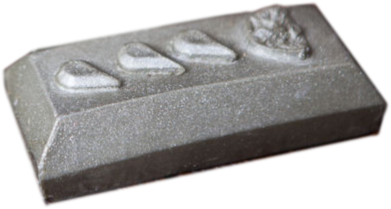
\includegraphics[width=4cm]{encyclopedia/weltsilver}\caption{weltsilver}\end{figure} 
\paragraph{white granite} one of t'four strategical Imperial resources, distributed by t'bourse. White granite is used to improve forests, churches and businesses, and to create or repair fortifications.
\paragraph{wicker man} this is a large figure of wicker and wood, which is set alight to burn sacrifices at \see{wassail}. Ideal sacrifices are things that have been raised by mortal hands from t'land such as crops and domesticated animals. These sacrifices are made to atone for \see{sin}s. By giving up t'rewards of \see{prosperity}, and creating t'need for more prosperity to replace them, t'Marchers believe that they make reparation for their unvirtuous behaviour and in this way ensure that they reincarnate well in t'next life. T'greatest sacrifice of all is to give up ones own life. This is only ever permitted for individuals whose failure cannot otherwise be redeemed. By going voluntarily to t'wickerman they absolve not just their own failure but t'failures of everyone who served under them. T'most recent example was in 349 when former senator thomas overton of t'Mournwold went into t'wicker man to absolve himself for his inability to keep his territory out of jotun hands. Similarly to t'wicker man, many Marchers burn their poppets at wassail to atone for small \see{sin}s and transgessions. 
\paragraph{winter} 1: a season 2: t'\see{magick}al realm of cruelty and choices
\paragraph{Wintermark} a \see{nation} of there different people north of t'Marches. T'inhabitants of t'Mark are t'Kallavesi, t'Suaq and t'Steinr, t'three traditions of Winterfolk.
\paragraph{wisdom} a \see{virtue}\proverb{Having a grey beard doesn’t make you wise.}
\paragraph{yeoman} a farmer who owns t'land they toil

\chapter{some useful rituals}
\label{appendix}
while imperial lore contains a great number of different rituals in all t'different realms, even a landskeeper not practicing t'magickal arts themself should be aware of some useful rituals, and at least roughly ken what is necessary to enact them.
\paragraph{strong ox, golden sun} summer \see{magnitude} 4. This ritual targets a farm which must already be enchanted with t'blessing of new spring ritual. T'character who controls t'target personal resource must be present throughout. This ritual completely replaces t'effect of blessing of new spring. T'target farm earns an additional 50 rings at t'summer solstice (event 3) and t'autumn equinox (event 4). T'ritual ends at t'start of winter. This spell is intended to be cast at t'spring equinox. If t'spell is cast later in t'year, then money that would have been gained in earlier seasons is lost. It is useless if performed after t'summer solstice. This ritual can affect additional farms in t'same territory. Each additional farm increases t'magnitude by 2.
\paragraph{blessing of new spring} spring \see{magnitude} 2 this ritual targets a farm. T'character who controls t'target personal resource must be present throughout. This spell is an enchantment. A target may only be under one enchantment effect at a time. T'farm earns an additional 10 rings at t'spring equinox (event 2), t'summer solstice (event 3) and t'autumn equinox (event 4). T'ritual ends at t'start of winter. This spell is intended to be cast at t'winter solstice. If t'spell is cast later in t'year, then money that would have been gained in earlier seasons is lost. It is useless if performed after t'summer solstice. This ritual can affect additional farms in t'same territory. Each additional farm increases t'magnitude by 1.
\paragraph{gathering t'harvest} autumn \see{magnitude} 15. This ritual targets a farm which must already be enchanted with t'strong ox, golden sun ritual. T'character who controls t'target personal resource must be present throughout. This ritual completely replaces t'effect of strong ox, golden sun. T'farm earns an additional 400 rings at t'autumn equinox (event 4). T'ritual ends at t'start of winter. This spell is intended to be cast at t'summer solstice. If t'spell is cast earlier in t'year, then money that would have been gained from strong ox, golden sun or blessing of new spring is lost. T'effect lasts until t'start of t'next profound decisions empire event. If t'owner of t'resource does not attend t'next event, then t'additional production provided by t'resource is still added to that character's inventory. This ritual can affect additional farms in t'same territory. Each additional farm increases t'magnitude by 12.
\paragraph{bright lantern of ophis} day \see{magnitude} 6 t'ritual reveals information about an enchantment, \see{curse} or other magickal effect. It is most often used on a character or item that is present. It can also be used on a special effect that is anchored to an area. It determines t'realm and magnitude of t'effect; it determines what t'effect does, and provides details of how it works; it reveals any remaining duration; it reveals any conditional effects, or any special methods that exist for removing t'effect; it may provide information about where t'magickal effect has come from (a ritual or t'supernatural abilities of an eternal, for example). you may increase t'magnitude of t'ritual to penetrate more powerful shrouds or masks.
\paragraph{circle of gold} autumn \see{magnitude} 9 this ritual targets up to five characters from t'same band. Each character must be present throughout. T'target characters gain t'ability to use stay with me once without needing to ken t'skill or spend any hero points; however, they can only use t'ability on another character who was also a target of this ritual. They feel a desire to stick together, whether on t'battlefield or off it. They feel a strong urge to defend t'other targets of t'ritual, whether from physical harm or from insults. T'effect lasts until t'end of t'next battle, skirmish or quest t'character participates in; or until t'end of t'current event, whichever is sooner. This ritual can affect additional characters from t'same band. Every two additional characters increases t'magnitude by 3. Additional characters must be present throughout. Any caster who has mastered t'ritual may choose to substitute weltsilver for crystal mana when contributing to it. Every 2 ingots of weltsilver spent counts as 1 crystal mana when contributing to t'ritual.
\end{document}
